\documentclass[openany]{article}
%\usepackage[english]{babel}
\usepackage[spanish,es-tabla,activeacute]{babel}
\usepackage{commands}
\usepackage{xcolor}

\usepackage{lipsum}
\usepackage{algorithm}
\usepackage{algpseudocode}
\usepackage{float}
\usepackage{svg}
\usepackage{multirow}

\pagestyle{fancy}
\fancyhf{}
\lhead{}
\rhead{\leftmark}
\cfoot{\thepage}

\setlength{\parskip}{4mm}

\addbibresource{references.bib}

% Cambiar "Algorithm" por "Algoritmo" en el título del algoritmo
\makeatletter
\renewcommand{\ALG@name}{Algoritmo}
\makeatother


\begin{document}

\counterwithout{equation}{section}

\thispagestyle{empty}

\begin{titlepage}
    \begin{figure}[th]
        \begin{flushleft}
            
\includegraphics[width=7cm]{Figures/image1.png}
            
\includegraphics[width=4cm]{Figures/valgrai.jpeg}
        \end{flushleft}
    \end{figure}
    \vspace{1cm}

    {\flushleft \LARGE \bfseries TRABAJO DE FIN DE MÁSTER\par}\vspace{2cm}

    % Thesis title
    {\flushright \LARGE \bfseries Optimización del llenado manual de contenedores con paquetes heterogéneos  \par}\vspace{2cm}

    {\flushleft \LARGE \bfseries Jose Gustavo Quilca Vilcapoma \par}\vspace{1cm}

    {\flushleft \Large \bfseries Tutor: Javier Alcaraz Soria \par}\vspace{1.5cm}

    {\flushleft \bfseries Máster Universitario en Estadística Computacional y Ciencia de Datos para la Toma de Decisiones\par}\vspace{0.cm}
    {\flushleft \bfseries Instituto Centro de Investigación Operativa\par}\vspace{1cm}

    {\flushleft \small \bfseries Curso 2023-2024\par}\vspace{2cm}

    \newpage\thispagestyle{empty}

    % Thesis title
    {\flushleft \LARGE \bfseries Optimización del llenado manual de contenedores con paquetes heterogéneos \par} \vspace{1.5cm}

    {\flushleft \LARGE \bfseries Jose Gustavo Quilca Vilcapoma \par}\vspace{1cm}

    {\flushleft \Large \bfseries Tutor: Javier Alcaraz Soria \par}\vspace{1.5cm}

    {\flushleft \Large \bfseries Máster Universitario en Estadística Computacional y Ciencia de Datos para la Toma de Decisiones\par}\vspace{0.cm}
    {\flushleft \Large \bfseries Instituto Centro de Investigación Operativa\par}\vspace{0.cm}
    {\flushleft \Large \bfseries Universidad Miguel Hernández de Elche\par}\vspace{0.cm}
    {\flushleft \small \bfseries Curso 2023/2024\par}\vspace{1.5cm}

    {\flushleft \normalsize Palabras clave:\par}\vspace{0cm}

    {Optimización, Problema de llenado de contenedores, Algoritmo Genético \par}
    \vspace{1.5cm}

\end{titlepage}

% \clearpage\thispagestyle{empty}\null\newpage %blank page

\pagenumbering{roman}
% \newpage
% \thispagestyle{plain}

% \mbox{}\par
% \vspace{4.5cm}

%\begin{flushright}
%    \textit{Insert comment here}
%\end{flushright}

% \clearpage\thispagestyle{empty}\null\newpage %blank page

\newpage
\thispagestyle{plain}
\section*{Agradecimientos}

\lipsum[0]
Quiero expresar mi más profundo agradecimiento a mi tutor, Javier Alcaraz, por el enorme interés que ha mostrado en este proyecto. Sus consejos y valoraciones fueron fundamentales para el desarrollo de este trabajo. Asimismo, agradezco al instituto CIO y a todos los profesores por proporcionarnos los conocimientos necesarios para ejercer esta profesión. Mi gratitud también va dirigida a la institución Valgrai por su apoyo con la beca de estudios. A mis compañeros, gracias por sus valiosos consejos y apreciaciones. Y, por último, a mi familia, agradezco de corazón toda la paciencia y el apoyo brindado durante este tiempo.

\mbox{}\par
\vspace{0.5cm}

\begin{flushright}
    \textit{Jose Gustavo Quilca Vilcapoma}
\end{flushright}


% \clearpage\thispagestyle{empty}\null\newpage %blank page

\newpage
\thispagestyle{plain}

\section*{Abstract}

For many years, the use of containers for transporting goods has been a fundamental part of international trade. However, this process involves high costs and generates a considerable carbon footprint. Therefore, optimizing the loading of these containers would help mitigate these negative effects. This work focuses on the optimization of container loading, a widely studied problem considered NP-hard in combinatorics. Additionally, realistic constraints that affect the final arrangement of packages in the container, arising from the need for manual loading, are taken into account. To address this problem, the use of a metaheuristic method based on a genetic algorithm, adapted along with a loading imitation, is proposed. Improvements in the loading process that increase the efficiency of the algorithm are also suggested. In order to demonstrate the effectiveness of the proposals, several experiments are conducted to compare performance with different package configurations, thus offering an effective solution to this logistical challenge of container loading with heterogeneous packages.

\vspace{2cm}

\section*{Resumen}

Desde hace muchos años, el uso de contenedores para el transporte de mercancías ha sido una parte fundamental del comercio internacional. Sin embargo, este proceso implica costos elevados y genera una huella de carbono considerable. Por ello, optimizar la carga de dichos contenedores ayudaría a mitigar estos efectos negativos. Este trabajo se centra en la optimización del llenado de contenedores, un problema ampliamente estudiado y considerado de tipo NP-duro en combinatoria. Además, se tienen en cuenta restricciones realistas que afectan la disposición final de los paquetes en el contenedor, surgidas de la necesidad de un llenado manual. Para abordar este problema, se propone el uso de un método metaheurístico basado en un algoritmo genético, adaptado junto a una imitación del proceso de llenado. También se sugieren mejoras en el proceso de llenado que incrementan la eficiencia del algoritmo. Con el fin de demostrar la efectividad de las propuestas, se llevan a cabo varios experimentos que permiten comparar el desempeño con distintas configuraciones de paquetes, ofreciendo así una solución eficaz a este desafío logístico del llenado de contenedores con paquetes heterogéneos.

\addcontentsline{toc}{section}{\protect\numberline{}Abstract}%

% \clearpage\thispagestyle{empty}\null\newpage %blank page

% \newpage
% \thispagestyle{plain}

% \section*{Abbreviations}

% \textbf{LHS} Left Hand Side \\

% \textbf{MF} Mean-Field \\

% \textbf{RHS} Right Hand Side \\

% \textbf{MSE} Mean Squared Error

% \clearpage\thispagestyle{empty}\null\newpage %blank page

\newpage
\thispagestyle{plain}
{
    %\hypersetup{hidelinks}
    \tableofcontents
}


\thispagestyle{empty}

\clearpage\thispagestyle{empty}\null\newpage %blank page

\pagenumbering{arabic}

\newpage




\section{Introducción} \label{sec: introducción}

En el comercio internacional, el transporte de mercancías se realiza principalmente a través de contenedores de carga. Los contenedores son cajas de acero de forma rectangular que se utilizan para transportar mercancías en barcos, trenes y camiones. Los contenedores son una forma eficiente y segura de transportar mercancías, ya que permiten que las mercancías se carguen y descarguen rápidamente y se almacenen de manera segura durante el viaje. Los contenedores vienen en diferentes tamaños y capacidades, y se utilizan para transportar una amplia variedad de mercancías, incluyendo productos manufacturados, materias primas, alimentos, etc. Para un buen aprovechamiento del espacio y la capacidad de carga de los contenedores, es importante que las mercancías se carguen de manera eficiente y se aproveche al máximo el espacio disponible.

En muchos casos, estas mercancías se encuentran en cajas o paquetes de diferentes tamaños, formas y pesos. Optimizar el llenado de dichos paquetes en los contenedores es un problema importante en la industria de la logística y el transporte ya que puede tener un impacto significativo en los costos y la eficiencia de la cadena de suministro. Por otro lado el mejor aprovechamiento del espacio y la capacidad de carga de los contenedores puede ayudar a reducir el número de viajes necesarios para transportar las mercancías, lo que puede reducir los costos de transporte y las emisiones de carbono asociadas \parencite{Parreo2008AMA}.

El problema de llenado de paquetes en contenedores es un problema de optimización combinatoria que ha sido ampliamente estudiado en la literatura. Así mismo, problemas similares se pueden observar en distintas industrias, como el llenado de paquetes en camiones, carga de pallets, carga en almacenes, entre otros, donde la colocación de cajas dentro de otras cajas más grandes es una tarea que se realiza con frecuencia. El llenado de contenedores consiste en colocar paquetes de diferentes tamaños y formas en un contenedor de manera que se utilice el espacio disponible de la mejor manera posible, cumpliéndose ciertas restricciones (peso, estabilidad, etc.) y optimizando uno o más objetivos, entre los que puede estar el minimizar el espacio no utilizado o maximizar el beneficio asociado a la carga transportada, por poner sólo algunos ejemplos. Este problema ha sido clasificado como NP-duro \parencite{PISINGER2002382}, lo que significa que muchas veces para instancias grandes de paquetes no existe un algoritmo de tiempo polinomial que pueda resolverlo de manera exacta. Por ello, muchos autores han propuesto diferentes enfoques heurísticos y metaheurísticos para resolver este problema de manera aproximada.

Existen diferentes variantes del problema de la carga de contenedores con paquetes, dependiendo de las restricciones y objetivos específicos que se consideren. Algunas de las variantes más estudiadas incluyen el uso de paquetes homogéneos, paquetes heterogéneos, paquetes rotativos, paquetes frágiles, entre otros. En este trabajo, nos enfocaremos en restricciones derivadas de un caso de uso real que se da cuando la carga es realizada por uno o varios operarios, es decir una carga manual, cuyo principal objetivo es facilitar el proceso de la carga poniendo énfasis en las limitaciones que un operador humano pueda tener. Para esto se considera el uso de paquetes de baja heterogeneidad, que consiste en grupos de paquetes que comparten ciertas características, como el tamaño, el peso, el beneficio, es decir, paquetes que pueden ser cargados por una persona sin necesidad de maquinaria. También consideraremos restricciones de rotación, que indican que los paquetes pueden ser girados en ciertas direcciones para aprovechar mejor el espacio disponible y restricciones de contigüidad, que indican que los paquetes del mismo grupo deben ser cargados de manera contigua.

En este trabajo, se propone una metaheurística basada en el algoritmo genético para resolver el problema de la carga manual de contenedores con paquetes heterogéneos. El algoritmo genético es una técnica de optimización que se basa en la evolución biológica y que ha sido ampliamente utilizada para resolver problemas de optimización combinatoria. El algoritmo genético es un enfoque de búsqueda poblacional que mantiene una población de soluciones candidatas y utiliza operadores genéticos como la selección, el cruce y la mutación para generar nuevas soluciones a partir de las soluciones existentes. El algoritmo genético es un enfoque flexible y versátil que ha demostrado ser efectivo para resolver una amplia variedad de problemas de optimización combinatoria.

Para evaluar las soluciones que el algoritmo genético va generando, se ha implementado un algoritmo que imita el llenado manual que realizaría un operario, teniendo en cuenta todos los condicionantes que supone este proceso. Por ejemplo, el operario no puede alcanzar ciertas zonas del contenedor si no hay espacio suficiente para pasar o si otros paquetes que han sido colocados anteriormente le obstruyen el paso.

Este trabajo se enfoca en resolver el problema de llenado de contenedores considerando un único contenedor y paquetes débilmente heterogéneos, esta clasificación también es conocida como Three-dimensional Single Large Object Placement Problem (SLOPP) cuya clasificación fue propuesta por \textcite{WASCHER20071109}, sin embargo muchos de los trabajos en la literatura que resuelven este problema no consideran todas restricciones prácticas que se presentan en la industria. \textcite{SAFAK2023106199} también mencionan que encontrar una disposición óptima de los paquetes en los contenedores mientras se satisfacen una variedad de restricciones del mundo real es una tarea no trivial.

Con esta falta de enfoques en la literatura con un conjunto realista de restricciones prácticas, nuestro objetivo es proponer un método metaheurístico de buen rendimiento que sea capaz de resolver problemas con un razonable número de paquetes y garantizar resultados consistentes de buena calidad. Consideramos las restricciones prácticas que tienen como origen del hecho de ser un llenado manual de los paquetes en el contenedor. El método de solución propuesto consiste en un enfoque de llenado priorizando el espacio más al fondo, más debajo y más a la izquierda, compuesto por un imitación del llenado realizado por el ordenador y unas propuestas de mejoras en los procesos de llenado. El método está estructurado de tal manera quede claro y facilite el procedimiento de carga para el operario.

Las contribuciones de este trabajo son las siguientes:

\begin{itemize}
    \item Se propone un método de solución basado en una metaheurística de buen rendimiento para resolver el problema de llenado de contenedores con un conjunto realista de restricciones prácticas derivadas de un caso de uso real de carga manual.
    \item Se propone una mejora en el proceso de llenado que ayuda a la metaheurística a encontrar soluciones de mejor calidad en menos tiempo.
    \item Se presenta una serie de experimentos computacionales que muestran la eficacia del método propuesto en diferentes instancias del problema.
\end{itemize}

El resto de este trabajo está organizado de la siguiente manera. En la sección 2, se presenta una revisión de la literatura relacionada con el problema de la carga de contenedores y sus variantes. En la sección 3, se presenta la definición formal detallada y formal del problema planteado. En la sección 4, se describe la metaheurística propuesta para resolver el problema. En la sección 5, se presenta un estudio computacional para evaluar el desempeño con diferentes configuraciones. Finalmente, en la sección 6, se presentan las conclusiones y las direcciones futuras de investigación.





\newpage






\numberwithin{equation}{section}

\section{El problema de la carga de contenedores: Revisión de la literatura}

El problema de llenado de paquetes en contenedores es también conocido en la literatura como Container Loading Problem o CLP, ha sido ampliamente estudiado desde los años 60's \parencite{barnett1967exact}, una de las definiciones más sencillas lo realiza \textcite{GEORGE1980147} quién lo define como encontrar posiciones adecuadas para colocar las cajas en el contenedor de tal manera que todas las cajas puedan ser colocadas en el contenedor sin superponerse de tal modo que se maximice la utilización del espacio. Existe mucha literatura respecto a este problema. A continuación presentamos un resumen de la misma, haciendo hincapié en que hay muy diversas variantes del problema.

El problema de llenado de contenedores tiene su origen en el campo del transporte y la logística. Surge de la necesidad de empacar eficientemente objetos en contenedores o vehículos mientras se optimiza la utilización del espacio. Aunque tiene un origen en la industria, el problema ha sido ampliamente objeto de investigación en la comunidad académica, debido a su complejidad, quienes también los clasifican como un problema de optimización combinatoria derivado de otros problemas de optimización como el problema de cortes y empacado de objetos \parencite{Alvarez-Valdes2018} o el problema de la mochila \textcite{DEQUEIROZ2012200} entre otros.

Existen muchos tipos de problemas de llenado de contenedores, presentaremos a continuación algunas de las clasificaciones más comunes que se han propuesto en la literatura.

Muchos de los tipos de problemas formulados en torno al CLP pueden categorizarse en dos tipos principales, los problemas de llenado con restricciones básicas y los problemas de llenado con restricciones prácticas o reales. Los problemas con restricciones básicas son aquellos que consideran restricciones simples, por ejemplo, que los paquetes no pueden ser superpuestos y que deben ser colocados dentro de los límites del contenedor, también llamado restricciones de viabilidad del empaquetado \parencite{scheithauer2017introduction}. Los problemas con restricciones prácticas consideran restricciones más realistas como por ejemplo, restricciones de estabilidad, restricciones de rotación, restricciones de contigüidad o restricciones de peso, entre otras \parencite{KURPEL202087}.

\textcite{Bortfeldt20131} hicieron una revisión de las distintas variantes, en función de las restricciones consideradas en la literatura, entre las que se encuentran:

\textbf{CLP con múltiples contenedores}: También conocido como el problema de llenado de contenedores múltiples, es una variante del CLP en la que se tienen varios contenedores y se busca llenarlos con un conjunto de paquetes. El objetivo es minimizar el número de contenedores utilizados, maximizando la utilización del espacio en los contenedores.

Algunas de las subvariantes de este problema incluyen el uso de contenedores del mismo tamaño o de diferentes tamaños, por ejemplo, Single Bin-Size Bin Packing Problem (SBSBPP) se enfoca en llenar un conjunto de contenedores de un solo tamaño con un conjunto de paquetes \parencite{ren2011priority}, mientras que Multiple Bin-Size Bin Packing Problem (MBSBPP) se enfoca en llenar un conjunto de contenedores de diferentes tamaños con un conjunto de paquetes \parencite{zhao2016comparative}.

\textbf{CLP con restricciones de estabilidad}: La estabilidad se refiere a la capacidad de los paquetes de mantenerse en su lugar ya sea en reposo o durante el transporte, evitando movimientos no deseados que puedan dañar la carga o el contenedor. Las restricciones de estabilidad se refieren a las condiciones que deben cumplirse para garantizar que la carga sea estable, como por ejemplo, que los paquetes no se aplasten, no se deslicen y no se caigan.

\textcite{Bortfeldt20131} identifican dos variantes en función de las restricciones de estabilidad: estática y dinámica, señalando que la mayoría de los estudios se concentran en la primera y pocos en la estabilidad dinámica. Critican las métricas de estabilidad existentes por ser insuficientes y no reflejar adecuadamente la estabilidad dinámica real, lo que puede llevar a evaluaciones incorrectas.

\textcite{RAMOS2015480} proponen un enfoque para determinar métricas de estabilidad más realistas y aborda la importancia de la estabilidad en las operaciones de carga de contenedores, destacando su impacto en la satisfacción del cliente, la eficiencia operacional y la seguridad de los paquetes junto a la de los operarios.


\textbf{CLP con restricciones de rotación}: Las restricciones de rotación se refieren a la capacidad de los paquetes de ser rotados en diferentes direcciones, lo que puede aumentar la utilización del espacio y mejorar la estabilidad de la carga. \textcite{Bortfeldt20131} señalan que es un tipo de restricción común en la literatura y que se ha investigado ampliamente, categorizando las restricciones de rotación en 6 tipos:

\begin{itemize}
    \item Caso 1: No se permite rotar las cajas, que deben colocarse en una única orientación fija tanto vertical como horizontalmente.
    \item Caso 2: Solo se permite una orientación vertical fija para cada tipo de caja, pero se pueden rotar 90° en el plano horizontal.
    \item Caso 3: Las cajas pueden rotarse libremente en el plano horizontal y tienen restricciones limitadas en la orientación vertical.
    \item Caso 4: Las cajas pueden tener hasta cinco orientaciones prohibidas en cualquier dirección, permitiendo una amplia variedad de restricciones.
    \item Caso 5: Todas las cajas son completamente rotativas sin restricciones de orientación, proporcionando el máximo grado de libertad.
\end{itemize}

\textbf{CLP con paquetes heterogéneos}: La heterogeneidad de los paquetes se refiere a la variabilidad en las dimensiones, formas y pesos de los paquetes, lo que puede complicar el proceso de empaquetado y afectar la utilización del espacio. \textcite{WASCHER20071109} clasificaron los problemas de llenado de contenedores según la variedad de artículos grandes y pequeños, relacionándolo con el número de diferentes tipos de artículos en el problema y lo clasificaron como: homogéneo (un solo tipo), fuertemente heterogéneo (muchos tipos) o ligeramente heterogéneo (pocos tipos).

\textcite{zhao2016comparative} propusieron una clasificación más detallada basada en la homogeneidad de los contenedores y las cajas, identificando seis subtipos de problemas de llenado de contenedores:

\begin{itemize}
    \item Problema de corte de stock de tamaño único (SSSCSP) si los contenedores son idénticos y las cajas son ligeramente heterogéneas.
    \item Problema de empaque de contenedor de tamaño único (SBSBPP) si los contenedores son idénticos y las cajas son muy heterogéneas.
    \item Problema de corte de stock de múltiples tamaños (MSSCSP) si tanto los contenedores como las cajas son ligeramente heterogéneos.
    \item Problema de empaque de contenedor de múltiples tamaños (MBSBPP) si los contenedores son ligeramente heterogéneos y las cajas muy heterogéneas.
    \item Problema de corte de stock residual (RCSP) si los contenedores son muy heterogéneos y las cajas ligeramente heterogéneas.
    \item Problema de empaque de contenedor residual (RBPP) si tanto los contenedores como las cajas son muy heterogéneos.
\end{itemize}

\subsection{Metodologías de solución}

Muchos autores han propuesto diferentes enfoques para resolver este problema de manera exacta o aproximada. A continuación se presentan algunas de las metodologías de solución que se han propuesto en la literatura.

\textbf{Métodos exactos}: Los métodos exactos son aquellos que garantizan encontrar la solución óptima al problema, sin embargo, estos métodos pueden ser computacionalmente costosos y no escalables para problemas grandes. Muchos autores han intentado resolver el CLP con restricciones prácticas de manera exacta, pero la mayoría ha encontrado que los métodos exactos no son adecuados para problemas de gran tamaño. Por ejemplo, \textcite{JUNQUEIRA201274} mencionan que tuvieron problemas de desbordamiento de memoria al intentar resolver instancias con mas de 20 tipos. Más recientemente, \textcite{NASCIMENTO2021105186} propusieron un enfoque exacto basado en modelos de programación lineal entera y programación por restricciones para resolver el problema de llenado de contenedores, demostrando que pudieron resolver instancias de hasta 10 tipos de paquetes y hasta 110 paquetes en un tiempo razonable.

\textbf{Métodos heurísticos}: Los métodos heurísticos son aquellos que no garantizan encontrar la solución óptima, pero pueden proporcionar soluciones de buena calidad en un tiempo razonable. Los métodos heurísticos son ampliamente utilizados para resolver problemas de optimización combinatoria, como el CLP, debido a su eficiencia y escalabilidad. Algunos de los métodos heurísticos constructivos más comunes que se han propuesto en la literatura son: heurística en base a la construcción de paredes \parencite{GEORGE1980147}, con una versión mejorada por \textcite{PISINGER2002382} y heurística en base a la construcción por capas \parencite{BISCHOFF1995377}, con una versión mejorada por \textcite{RANCKJUNIOR2019471}.

\textbf{Métodos metaheurísticos}: El término metaheurística fue acuñado en los años 80s por \textcite{GLOVER1986533}. Una metaheurística puede entenderse como una metodología que incluye estrategias maestras capaces de guiar la búsqueda hacia la solución óptima global. Se consideran más complejas y eficientes que los algoritmos heurísticos simples porque exploran áreas en el espacio de soluciones que van más allá de las exploradas por las heurísticas simples, las cuales tienden a centrarse en encontrar una única solución óptima local. Luego \textcite{Sorensen2013} lo definieron como "Un marco algorítmico de alto nivel e independiente del problema que proporciona un conjunto de directrices o estrategias para desarrollar algoritmos de optimización heurísticos". Más recientemente, \textcite{MARTI2024} definen una metaheurística no como un algoritmo específico con pasos precisamente definidos, sino como un conjunto más o menos consistente de ideas de alto nivel. Estas ideas sirven como directrices para desarrollar algoritmos de optimización heurísticos ajustados a problemas específicos. En esta definición, se enfatiza la flexibilidad que tiene el diseñador del algoritmo para elegir las características específicas de su método, y se destaca que puede requerirse un grado considerable de "ingeniería" para adaptar el marco de metaheurística a fin de resolver problemas de optimización concretos.

Algunos de los métodos metaheurísticos más comunes que se han propuesto en la literatura para resolver el problema de llenado de contenedores son:

\begin{itemize}
    \item \textbf{Algoritmos Genéticos (GA)}: Se describe como un algoritmo de búsqueda inspirado en la evolución natural \parencite{goldberg2013genetic}, útil para resolver muchos problemas de optimización debido a su robustez y capacidad de manejar complejidades diversas. Los GA se utilizan en el contexto del CLP para manejar restricciones como el equilibrio de carga, considerado como una restricción estricta en algunos estudios. Por ejemplo, algunos autores que han usado GA para resolver el problema de llenado de contenedores son \textcite{RAMOS20181140}, \textcite{GONCALVES2012179}, \textcite{KANG20121287} entre otros.
    \item \textbf{Algoritmos de Enjambre de Partículas (PSO)}: Se describe como un algoritmo de optimización basado en la inteligencia de enjambre, como el de los pájaros o peces. Por ejemplo, algunos autores que han usado PSO para resolver el problema de llenado de contenedores son \textcite{KUO2023110417}, \textcite{domingo2012particle}, \textcite{Cano2010} entre otros.
\end{itemize}

\subsection{Software usado en la industria}

En la industria existen varios paquetes de software que permiten resolver el problema de llenado de contenedores, algunos de los más conocidos son:

\textbf{Cargo Manager}: Según \textcite{zhao2017three}, Cargo Manager (CM) es un ejecutable independiente diseñado para empaquetar contenedores siguiendo un orden de prioridad específico, comenzando por la parte trasera del contenedor. El proceso de empaquetado utiliza una serie de reglas de colocación, probando cada artículo en el orden establecido; si un artículo no es adecuado, se pasa al siguiente, volviendo a considerar los artículos no adecuados en futuras colocaciones. Los artículos de mayor prioridad se empaquetan primero y es posible configurar el sistema para que se adhiera estrictamente a las prioridades de empaque, asegurando que todos los artículos de una prioridad actual se empaquen antes de comenzar con la siguiente.

El proceso principal de empaquetado en CM utiliza diferentes métodos heurísticos constructivos que varían desde heurísticas básicas hasta métodos más complejos y consumidores de tiempo. El objetivo es maximizar el uso del espacio del contenedor formando "muros" con los artículos, donde cada bloque consiste en cajas del mismo tipo y orientación. A medida que se colocan los artículos, los espacios que ocupan ya no están disponibles, generándose nuevos espacios cúbicos que pueden fusionarse con espacios previos. Los métodos difieren en cómo seleccionan los espacios y las cajas, y las restricciones aplicadas al tamaño de los bloques.

En una etapa adicional, CM utiliza la heurística más básica para intentar empaquetar tantos artículos restantes como sea posible. Esta etapa no es adecuada para problemas de múltiples destinos o donde se requiere nivelación de carga, y excluye artículos pesados o frágiles. La solución óptima se determina comparando el volumen y la longitud utilizados por diferentes métodos, seleccionando como mejor aquella solución que ocupe mayor volumen o, en caso de igual volumen, utilice menos longitud. Los usuarios pueden decidir cuántas heurísticas se evalúan, y en caso de seleccionar un solo método, su solución se convierte automáticamente en la solución final. En la imagen \ref{fig:cargomanager} se muestra la interfaz gráfica de Cargo Manager.

\begin{figure}[H]
    \centering
    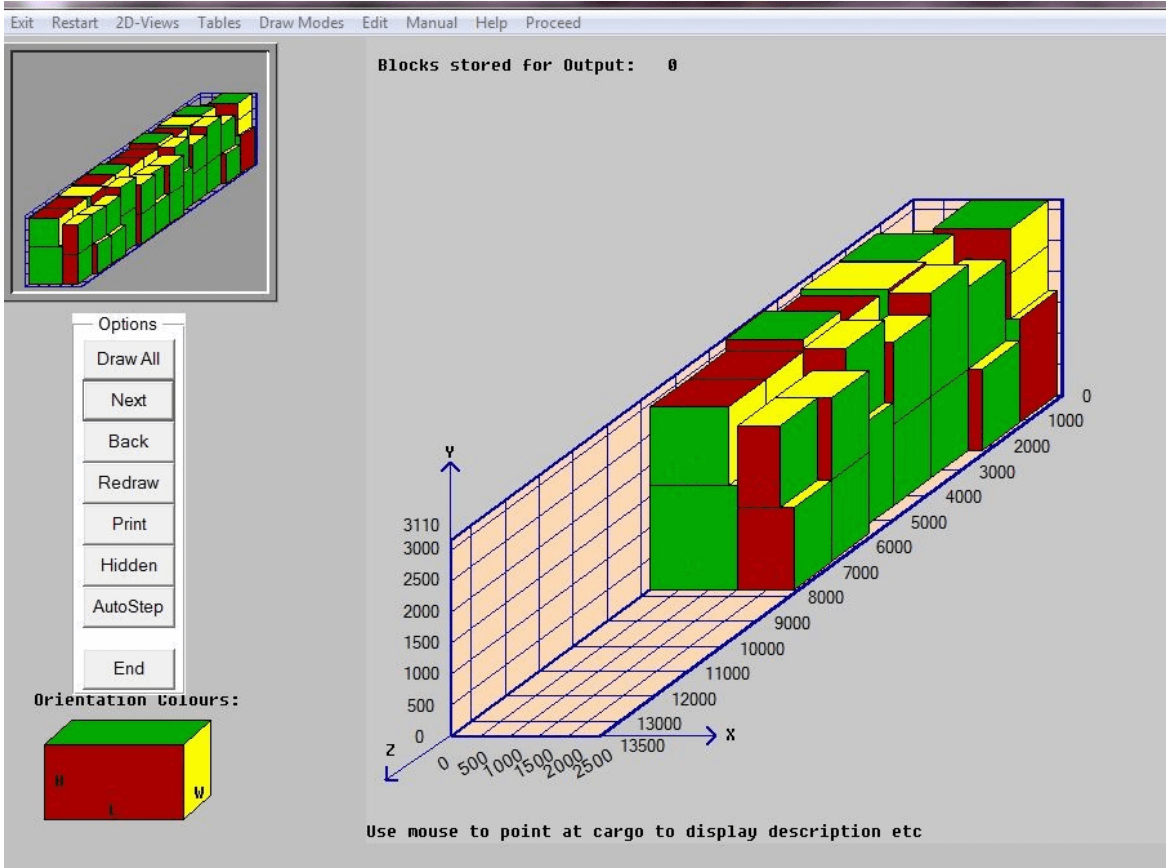
\includegraphics[width=0.5\textwidth]{Figures/cargomanager.png}
    \caption{La interfaz gráfica de Cargo Manager permite a los usuarios empaquetar contenedores siguiendo un orden de prioridad específico, maximizando el uso del espacio y minimizando la longitud utilizada \parencite{zhao2017three}.}
    \label{fig:cargomanager}
\end{figure}

\textbf{PackageCargo}: PackageCargo es una herramienta de apoyo a la decisión, diseñada para abordar el problema de carga de contenedores (CLP), que es esencial en la logística de transporte \parencite{MARTINEZFRANCO2020100601}. Desarrollada como una aplicación de código abierto usando el motor de juegos Unity, esta herramienta permite calcular, visualizar y guardar patrones eficientes de empaque, además de estimar métricas de estabilidad de la carga mediante modelos matemáticos y simulaciones físicas. Su objetivo principal es ofrecer un sistema utilizable tanto en entornos industriales como académicos, permitiendo a los usuarios modificar el marco de trabajo según sus necesidades, lo que ahorra tiempo en desarrollo de software y fomenta la contribución comunitaria para su mejora continua.

El software utiliza un diseño modular que incluye componentes para la visualización de soluciones, simulación de la estabilidad de la carga, y optimización de los patrones de empaque. La arquitectura de PackageCargo facilita la integración de algoritmos de optimización para generar patrones eficientes y su simulación correspondiente para evaluar la estabilidad, usando el motor de físicas PhysX de Nvidia. Esta estructura permite una fácil extensión y adaptación del software, fomentando la innovación y colaboración entre investigadores y profesionales del sector.

PackageCargo no solo ofrece una alternativa competitiva a soluciones comerciales, sino que también se posiciona como una plataforma valiosa para la investigación y el desarrollo en el ámbito del CLP. Al proporcionar una herramienta accesible y extensible, promueve el avance en la comprensión y solución de problemas complejos de carga, beneficiando tanto a la comunidad académica como a la industrial. En la imagen \ref{fig:packagecargo} se muestra la interfaz gráfica de PackageCargo.

\begin{figure}[H]
    \centering
    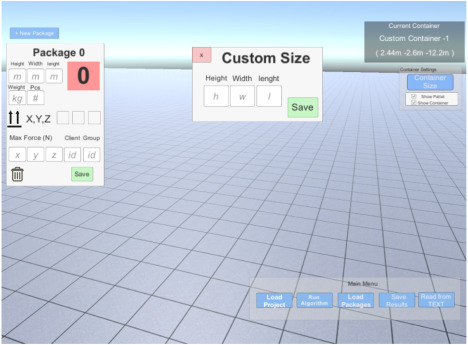
\includegraphics[width=0.6\textwidth]{Figures/packagecargo.jpg}
    \caption{La interfaz gráfica permite al usuario definir variedades de carga, dimensiones, restricciones y cantidades. Esta información se convierte en un archivo de entrada para los algoritmos generadores de patrones de empaque \parencite{MARTINEZFRANCO2020100601}.}
    \label{fig:packagecargo}
\end{figure}


\textbf{LoadCargo}: LoadCargo es un software comercial diseñado para facilitar la planificación y optimización de la carga en contenedores y camiones. Utiliza tecnología en 3D para ofrecer visualizaciones interactivas que mejoran la precisión de las simulaciones de carga. Este sistema admite tanto planificaciones automáticas como manuales, proporcionando herramientas flexibles para diversos requerimientos logísticos \parencite{loadcargo2024}.

El software es accesible en múltiples plataformas a través de Adobe Air, compatible con sistemas operativos como Windows, Mac OS X y Linux. Soporta tanto unidades métricas como imperiales y se integra con sistemas EDI (Intercambio Electrónico de Datos) para facilitar la importación de datos. Además, incluye características como la visualización del centro de gravedad, exportaciones de planificaciones a varios formatos y herramientas para la construcción de pallets, entre otras.

LoadCargo es eficaz para optimizar el uso del espacio en contenedores y camiones, aunque mencionan que presenta limitaciones como la incapacidad de manejar cargas de formas irregulares o volúmenes muy altos de cajas. Sin embargo, para operaciones estándar, ofrece soluciones robustas que mejoran la eficiencia en la carga y reducen los costos operativos. En la imagen \ref{fig:loadcargo} se muestra la interfaz gráfica de LoadCargo.

\begin{figure}[H]
    \centering
    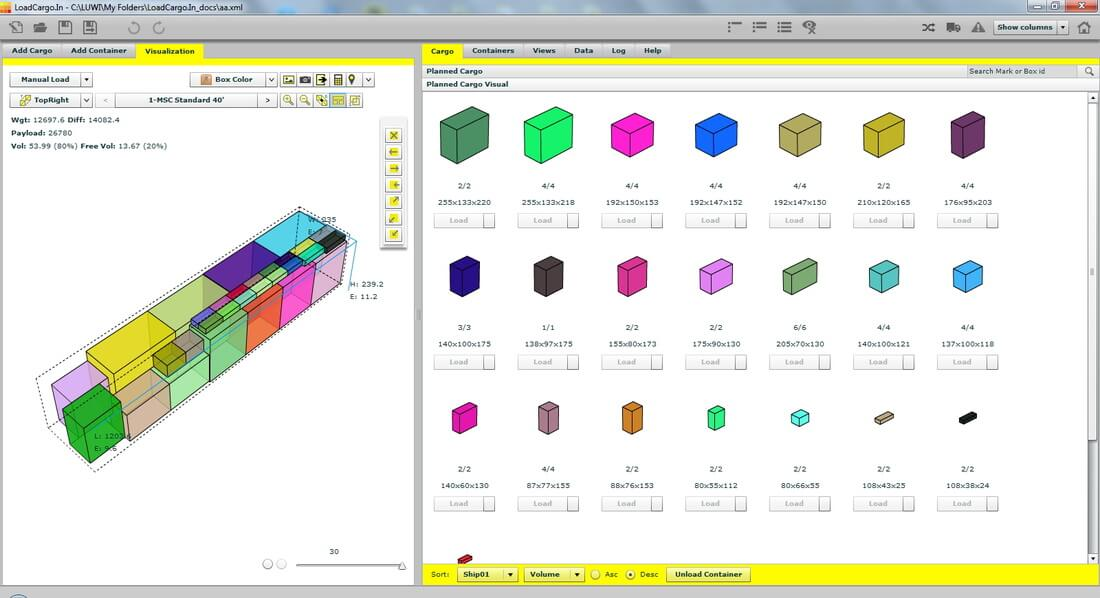
\includegraphics[width=0.6\textwidth]{Figures/loadcargo.jpg}
    \caption{La interfaz gráfica de LoadCargo permite a los usuarios visualizar y planificar la carga de contenedores y camiones, mejorando la eficiencia y reduciendo los costos operativos \parencite{loadcargo2024}.}
    \label{fig:loadcargo}
\end{figure}







\newpage



\section{Formulación del problema}
\label{sec:problem}

El problema planteado presentado se basa en una situación real relacionada con una empresa que gestiona un elevado volumen de pedidos de cajas de diferentes tipos. Cada semana, la empresa busca determinar cuántas cajas de cada tipo debe enviar en un contenedor para maximizar el beneficio total de dicho envío.

El desafío principal al que se enfrenta la empresa es optimizar el proceso de envío de cajas, donde cada una proporciona un beneficio específico. El problema consiste en determinar cómo utilizar de la mejor forma posible el espacio del contenedor para maximizar el beneficio. Dado que las cajas tienen distintos tamaños, pesos y beneficios, se plantea una dificultad para estimar de manera eficaz cómo llenar completamente un contenedor sin desperdiciar espacio. Este desperdicio no solo implica una pérdida financiera, sino que también tiene un impacto ambiental negativo, ya que cada viaje consume combustible y genera emisiones contaminantes.

Para abordar este desafío, es crucial considerar el proceso manual de carga del contenedor. El procedimiento actual de carga no está optimizado y no considera la disposición óptima de las cajas, lo que lleva a una carga subóptima y un desperdicio de espacio. Por tanto, es necesario revisar y mejorar este procedimiento para asegurar que se aproveche al máximo el espacio disponible en los contenedores.

El procedimiento de carga manual debe ser meticulosamente evaluado y optimizado. Este aspecto es crucial porque los operarios son los responsables de organizar físicamente las cajas en el contenedor. Un procedimiento manual de carga bien diseñado garantizaría que se aproveche cada centímetro disponible del contenedor, reduciendo así el espacio vacío y aumentando la rentabilidad del envío.

Respecto a las restricciones que se generan debido a la carga manual, se consideran las siguientes:

\begin{itemize}
    \item Los paquetes que son cajas de forma rectangular, pueden variar en tamaño, peso y beneficios, pero han sido concebidos previamente para que puedan ser cargados manualmente es decir que no son paquetes muy grandes o pesados.
    \item Los paquetes que comparten el mismo tamaño, peso y beneficio se consideran del mismo tipo, dos paquetes pueden tener el mismo tamaño y peso pero distinto beneficio, lo que los convierte en tipos diferentes. El beneficio de un paquete no depende de su tamaño o peso, es decir que un paquete sea más grande y pesado que otro no implica que sea de mayor beneficio y viceversa.
    \item Los paquetes llegan a la puerta del contenedor agrupados por tipo y en un orden específico, los paquetes pueden apilarse unos sobre otros independientemente de su tipo ya que las cajas lo soportan y sus pesos no son muy dispares, pero se debe asegurar la estabilidad de la carga. Por ejemplo, en el la Figura \ref{fig:paquetes_apilados} se muestra un ejemplo de cómo se apila un tipo de paquete encima de otro.
          \begin{figure}[H]
              \centering
              \includesvg[width=0.5\textwidth]{Figures/paquetes_apilados}
              \caption{Ejemplo de cómo se apila un tipo de paquete encima de otro.}
              \label{fig:paquetes_apilados}
          \end{figure}
    \item Para asegurar la estabilidad de la carga, un paquete más grande no puede estar encima de uno más pequeño, es decir un paquete siempre debe tener una base sobre la que se apoye. En la Figura \ref{fig:paquetes_mal_apilados} se muestra un ejemplo de una carga inestable.
          \begin{figure}[H]
              \centering
              \includesvg[width=0.5\textwidth]{Figures/paquetes_mal_apilados}
              \caption{Ejemplo de una carga inestable.}
              \label{fig:paquetes_mal_apilados}
          \end{figure}
    \item Para facilitar la carga manual se considera de que todos los paquetes de un mismo tipo deben mantener la misma orientación, es decir que no se pueden colocar paquetes de un mismo tipo en diferentes orientaciones, por ejemplo, en la Figura \ref{fig:paquetes_mal_orientados} se muestra un ejemplo de cómo no se deben colocar los paquetes, ya que dificultaría al operario seguir dicho procedimiento, además que aumentaría el riesgo de desperdiciar espacio o de que la carga sea inestable.
          \begin{figure}[H]
              \centering
              \includesvg[width=0.5\textwidth]{Figures/paquetes_mal_orientados}
              \caption{Ejemplo de cómo los paquetes de un mismo tipo tienen distinta orientación.}
              \label{fig:paquetes_mal_orientados}
          \end{figure}
    \item Muchas de las cajas están diseñadas para ser apiladas y soportar un gran peso encima siempre y cuando se respete la indicación de mantener una posición mirando hacia arriba, por lo que los paquetes solo pueden ser girados 90° en un solo eje, en cualquier dirección, por ejemplo, en la Figura \ref{fig:paquetes_girados} se muestra un mismo tipo de paquete girado en un eje.
          \begin{figure}[H]
              \centering
              \includesvg[width=0.5\textwidth]{Figures/paquetes_girados.svg}
              \caption{Ejemplo de dos paquetes de un mismo tipo, cada uno girado 90° con respecto al otro.}
              \label{fig:paquetes_girados}
          \end{figure}
    \item Para evitar la fatiga del operador por levantar los paquetes, la empresa suele usar cintas o bandas transportadoras, para aprovechar su uso, esto implica que los paquetes deben ser colocados en primer lugar lo más profundo posible del contenedor, es decir que los paquetes que están siendo cargados, deben ser colocados en la parte más alejada de la puerta del contenedor, de este modo también se evita que los paquetes obstruyan el ingreso del personal de carga al contenedor. En la Figura \ref{fig:cinta_transportadora} se muestra un ejemplo de cómo se puede hacer uso de una cinta transportadora que desliza los paquetes hacia el fondo del contenedor, mientras el contenedor se va llenando la cinta se va moviendo en sentido contrario.
          \begin{figure}[H]
              \centering
              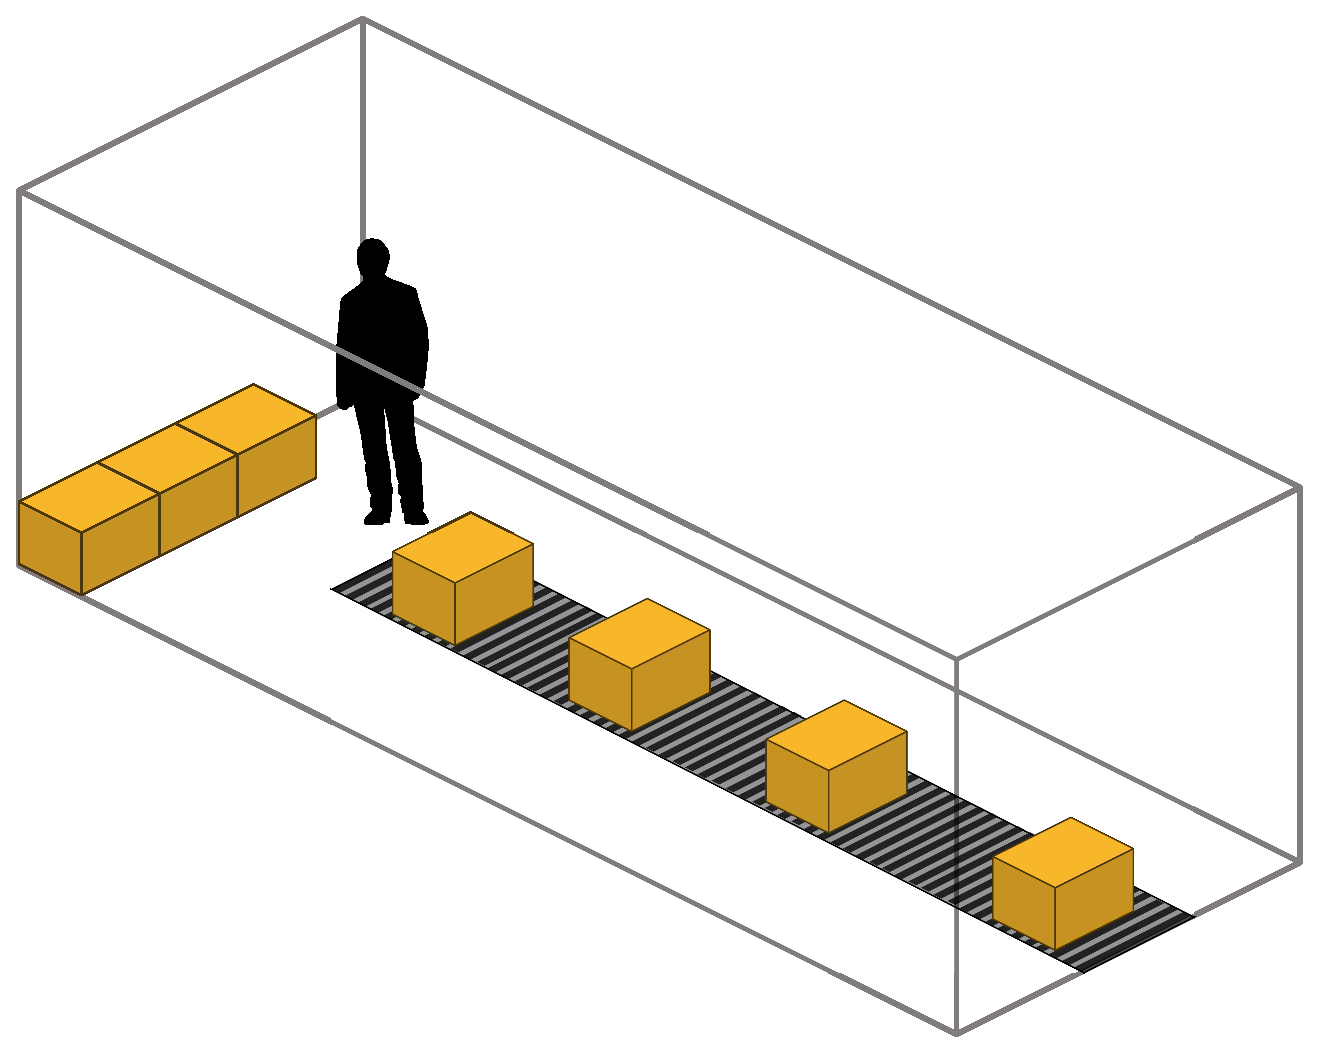
\includegraphics[width=0.5\textwidth]{Figures/cinta_transportadora.eps}
              \caption{Ejemplo del uso de una cinta transportadora.}
              \label{fig:cinta_transportadora}
          \end{figure}
    \item Las cajas se pueden apilar superiormente sin importar la altura alcanzada ya que los operadores cuentan con una pequeña escalera que les permite acceder a la parte más alta del contenedor.
\end{itemize}

Es importante destacar que se usa un procedimiento estandarizado para que el operario pueda elegir la posición de cada caja, priorizando los criterios dados a continuación:

\begin{itemize}
    \item La posición más profunda del contenedor, que ayuda a llenar primero los espacios más alejados de la puerta y evitar obstaculizar el ingreso del operador humano al contenedor.
    \item La posición más baja del contenedor, se da naturalmente debido al efecto de la gravedad, un paquete no podría ser colocado en una posición alta si no se ha llenado primero las posiciones más bajas.
    \item La posición más a la izquierda del contenedor, aunque no es una restricción fuerte, podría usarse el criterio de priorizar la posición más a la derecha si se considera necesario, lo crucial es mantener la consistencia al elegir una de estas dos direcciones. Para el caso de este trabajo se ha elegido la posición más a la izquierda.
\end{itemize}

El procedimiento de carga manual se basa en la combinación de las suposiciones, restricciones, reglas y criterios mencionados anteriormente, con el objetivo de lograr una carga eficiente y organizada de los paquetes en el contenedor. Este procedimiento asegura que se cumplan todas las condiciones establecidas.

El desafío que se enfrenta es conocer con anticipación la cantidad de paquetes por tipo que deben cargarse en el contenedor, así como definir el orden de carga y la rotación de cada tipo de paquete. El objetivo es lograr una disposición que no solo cumpla con las restricciones de espacio y los requerimientos del llenado manual, sino que también maximice el beneficio de la carga transportada.

\subsection{Definición formal del problema}

El problema de la carga manual de paquetes en un contenedor se define formalmente de la siguiente manera:

\begin{figure}[H]
    \centering
    \includesvg[width=0.4\textwidth]{Figures/container.svg}
    \caption{Contenedor con dimensiones $W$, $L$, $H$}
    \label{fig:container}
\end{figure}

Siendo un contenedor una caja de forma rectangular, de ancho $W$, largo $L$, alto $H$. En la figura \ref{fig:container} se muestra un contenedor con sus dimensiones, y una capacidad de carga $P$, se tiene definido unos tipos de paquetes también de formas rectangulares $t$, donde cada tipo $t$ pertenece a $T = \{0, 1, 2, \ldots, n\}$, además cada tipo $t$ posee ciertas dimensiones de ancho $w_t$, largo $l_t$, alto $h_t$, también posee un peso $p_t$ y un beneficio $b_t$, además se conoce la cantidad máxima $q^{max}_t$ de paquetes que dispone la empresa por cada tipo.

En este problema, consideramos que $W$, $L$, $H$ y $P$ , $w_t$, $l_t$, $h_t$, $p_t$, $q^{max}_t$ son enteros positivos, los cuales podrían ser representados en unidades de medida centímetros, milímetros.

\begin{figure}[H]
    \centering
    \includesvg[width=0.5\textwidth]{Figures/rotacion.svg}
    \caption{Rotación de un paquete en el eje $x$}
    \label{fig:rotation}
\end{figure}

Cada tipo de paquete, puede colocarse rotado o no, es decir, tendremos que determinar si $r_t \in \{0, 1\}$, debido al enfoque de carga manual, en el cual se establece que $\forall t$, $r_t \in \{0, 1\}$ donde $0$ representa que el tipo no se encuentra girado y $1$ que el tipo está girado 90° grados en el eje $x$, esto se puede ver en la figura \ref{fig:rotation} a) sin rotación y b) con rotación. Esto implica que los anchos y largos pueden intercambiarse, mientras que la altura no puede ser modificada.

La solución consiste en determinar para facilitar la carga manual, se debe disponer de un orden de carga $o_t$ para cada tipo $t$, donde $o_t \in O = \{0, 1, 2, \ldots, n\}$, que indica el orden en el que se debe cargar cada tipo de paquete en el contenedor.

La solución consiste en determinar la cantidad de paquetes por cada tipo a cargar $\tilde{q}_t$ (que no supere la cantidad máxima por tipo, $0 \leq \tilde{q}_t \leq q^{max}_t$) y el orden de carga de cada tipo $o_t$ con determinada rotación $r_t$, de tal modo que aplicando el procedimiento manual consigamos la mejor utilización posible del espacio. Además, se busca maximizar en primer lugar el beneficio total de la carga ($\max \sum_{t \in T} b_t \cdot \tilde{q}_t$) y en segundo lugar maximizar la utilización del espacio del contenedor ($\max \sum_{t \in T} w_t \cdot l_t \cdot h_t \cdot \tilde{q}_t$).

En el siguiente capítulo se presentará un algoritmo metaheurístico para resolver el problema de optimización de la carga manual de paquetes en un contenedor, considerando las restricciones de espacio del contenedor, así como las restricciones de rotación y orientación de los paquetes.








\newpage








\section{Metaheurística}

\subsection{Codificación de soluciones}
\label{sec:codificacion}

Existen diferentes maneras de codificar las soluciones para el problema de llenado de contenedores. Algunos de los más interesantes son por ejemplo, \textcite{GEHRING1997401}, que propusieron una codificación basada en listas dobles o simplemente dos listas de igual longitud, la primera representa la secuencia de llenado de los paquetes y la segunda indica la rotación de cada paquete.

Sin embargo, para las restricciones en nuestro problema, esta codificaciones no son adecuadas ya que necesitamos considerar que las cantidades de un tipo de paquete no son fijas sino que es algo a determinar como parte del problema. Por lo tanto, proponemos una codificación basada en tres listas de igual longitud, la primera lista representa la secuencia de llenado de cada tipo de paquete, la segunda lista indica la rotación de cada tipo de paquete y la tercera lista indica la cantidad de paquetes de cada tipo que se llenan en el contenedor.


Por ejemplo, si tenemos 4 tipos de paquetes $T=\{1,2,3,4\}$, todos los tipos con un mínimo de 0 paquetes y el tipo 1 con un máximo de 10 paquetes $q_1 \in [0,10]$, el tipo 2 con un máximo de 30 paquetes $q_2 \in [0,30]$, el tipo 3 con un máximo de 20 paquetes $q_3 \in [0,20]$ y el tipo 4 con un máximo de 22 paquetes $q_4 \in [0,22]$, una solución para el problema de llenado de contenedores podría ser la siguiente:

\begin{figure}[H]
    \centering
    \includesvg[width=0.4\linewidth]{Figures/codificacion.svg}
    \caption{Codificación de una solución con 4 tipos de cajas}
    \label{fig:codificación}
\end{figure}

La primera lista indica que el tipo 2 se llena primero, luego el tipo 1 seguido del tipo 4, y finalmente el tipo 3. La segunda lista indica que el tipo 2 no se rota, el tipo 1 se rota, el tipo 4 se rota y el tipo 3 no se rota. La tercera lista indica que se llenan 27 paquetes del tipo 2, 10 paquetes del tipo 1, 18 paquetes del tipo 4 y 13 paquetes del tipo 3.

Una ventaja de esta codificación es la flexibilidad que ofrece para adaptar el problema a diferentes restricciones, por ejemplo, si se desea considerar una cantidad fija de paquetes de un tipo, simplemente se puede fijar el mínimo y el máximo de ese tipo de paquete. De igual manera, la estructura soporta si se desea considerar otros tipos de rotaciones, además de las dos consideradas en el presente trabajo.

Este tipo de codificación permite representar soluciones factibles para el problema de llenado de contenedores, ya que considera la cantidad de paquetes de cada tipo que se llenan en el contenedor. Además, esta codificación es fácil de implementar y de entender, lo que facilita la implementación del algoritmo de llenado y del algoritmo de optimización para resolver el problema.

Para determinar si una solución es factible, es decir, si las cajas representadas caben mediante el proceso de llenado manual o no en el contenedor, debemos transformar dicha triple lista en un contenedor lleno de cajas, para lo cual nuestra función de evaluación imitará el proceso de llenado manual.

\subsection{Función de evaluación}

La función de evaluación es una parte fundamental de cualquier algoritmo de optimización, ya que permite evaluar la calidad de las soluciones generadas por el algoritmo y determinar si son factibles o no. Para el problema de llenado de contenedores, la función de evaluación se puede definir como la suma de los beneficios de los paquetes que se llenan en el contenedor, es decir, se busca maximizar el beneficio total de la carga que se llena en el contenedor.

Un paso previo importante antes de calcular el beneficio total de la carga es verificar si la solución generada es factible, es decir, si al agregar todas las cajas en los ordenes y las posiciones indicadas en la solución, se cumple que todas son colocadas en el contenedor sin superar su capacidad. Para ello, se propone un algoritmo que imita el procedimiento de llenado manual, el cual verifica si una solución generada es factible y si no lo es, lo corrige para que sea factible eliminando las últimas cajas sobrantes y modificando los genes correspondientes en el cromosoma que representa la solución.

\subsubsection{Algoritmo de llenado manual}

El algoritmo de llenado propuesto está basado en el método Deepest Bottom Left with Fill (DBLF) propuesto por \textcite{karabulut2004hybrid}, cuyo uso se ha extendido y varios autores han realizado propuestas para mejorarlo o adaptarlo a determinados contextos por ejemplo, \textcite{wang2010hybrid} y \textcite{kang2012hybrid}. El algoritmo propuesto en el presente trabajo está enfocado en cumplir las restricciones y adaptarse al contexto de un llenado manual de paquetes en un contenedor.

La idea básica del algoritmo DBLF es que los paquetes comienzan a ser llenados en el contenedor de forma secuencial, se prioriza que cada paquete se coloque en la posición más profunda (Deepest), mas baja (Bottom) y mas a la izquierda (Left) del contenedor.

Al inicio del procedimiento un paquete se coloca en el contenedor vacío siguiendo la prioridad DBL, luego al colocar el paquete en el contenedor, el espacio restante se divide en tres nuevos subespacios, la parte superior, la parte lateral y la parte frontal.

Es importante mencionar que existen diversas formas de dividir y formar estos nuevos tres subespacios, pero se elige una forma en específica, de modo que cumpla con las restricciones del llenado manual. En la figura \ref{fig:subespacios} se muestra de cómo se divide el espacio restante en el contenedor al colocar un paquete.

\begin{figure}[H]
    \centering
    \includesvg[width=0.9\textwidth]{Figures/subespacios.svg}
    \caption{División del espacio restante en el contenedor al colocar un paquete. a) Subespacio frontal, b) Subespacio lateral, c) Subespacio superior.}
    \label{fig:subespacios}
\end{figure}

Cada subespacio es considerado como un nuevo contenedor y se repite el proceso de colocar el siguiente paquete en uno de los subespacios creados. Para elegir el siguiente subespacio donde colocar el siguiente paquete, se usa el mismo criterio de priorización DBL, es decir, se elige el subespacio más profundo, más bajo y más a la izquierda, luego se coloca el paquete en dicho subespacio y se repite el proceso.

En la figura \ref{fig:segundo_paquete} se muestra un ejemplo de cómo se coloca un segundo paquete en el contenedor siguiendo el algoritmo DBLF.

\begin{figure}[H]
    \centering
    \includesvg[width=0.5\textwidth]{Figures/segundo_paquete.svg}
    \caption{Ejemplo de colocación de un segundo paquete en el contenedor luego de elegir el último subespacio lateral.}
    \label{fig:segundo_paquete}
\end{figure}

Para este segundo paquete, se ha elegido el anterior subespacio lateral, el cual fué el subespacio más profundo, más bajo y más a la izquierda, siguiendo el criterio de priorización DBL, luego se coloca el paquete en dicho subespacio y se repite el proceso de dividir el espacio restante. Como resultado de esta subdivisión, se obtienen en este caso solamente dos subespacios, la parte superior y la parte lateral, ya que no queda espacio frontal para dividir. En la figura \ref{fig:segundos_subespacios} se muestra estos dos nuevos subespacios.

\begin{figure}[H]
    \centering
    \includesvg[width=0.75\textwidth]{Figures/segundos_subespacios.svg}
    \caption{División del espacio restante en el contenedor al colocar un segundo paquete. a) Nuevo subespacio lateral, b) Nuevo subespacio superior.}
    \label{fig:segundos_subespacios}
\end{figure}

Este procedimiento se repite hasta que se hayan colocado todos los paquetes en el contenedor o no se pueda colocar más paquetes debido a restricciones de espacio. En la figura \ref{fig:contruccion_muro} se muestra como este procedimiento se asemeja a un tipo de construcción de un muro el cuál es otro método de llenado de contenedores.

\begin{figure}[H]
    \centering
    \includesvg[width=0.5\textwidth]{Figures/contruccion_muro.svg}
    \caption{Ejemplo de colocación de más paquetes en el contenedor}
    \label{fig:contruccion_muro}
\end{figure}

El Algoritmo \ref{alg:dblf} muestra el procedimiento de llenado manual de paquetes en un contenedor basado en el algoritmo DBLF.

\begin{algorithm}[H]
    \caption{Algoritmo de llenado manual de paquetes en un contenedor}
    \label{alg:dblf}
    \begin{algorithmic}[1]
        \State $Paquetes \gets \text{lista de paquetes}$
        \State \textbf{Inicialización:} $dblf \gets \text{lista inicializada con el espacio total del contenedor}$
        \State $Contenedor \gets \text{lista vacía para almacenar los paquetes colocados}$
        \For{$paquete \in Paquetes$}
        \State $SubespacioOptimo \gets \text{buscar el subespacio más adecuado en } dblf$
        \If{$SubespacioOptimo \neq \text{null}$}
        \State $Contenedor.\text{add}( \text{colocar}(paquete, SubespacioOptimo) )$
        \State $NuevosSubespacios \gets \text{dividir}(SubespacioOptimo, paquete)$
        \State $dblf.\text{remove}(SubespacioOptimo)$
        \State $dblf.\text{extend}(NuevosSubespacios)$
        \Else
        \State \textbf{print} $\text{"No se encontró espacio para el paquete."}$
        \EndIf
        \EndFor
        \State \Return $Contenedor$
    \end{algorithmic}
\end{algorithm}

El el Algoritmo \ref{alg:dblf}, en la línea 1: se inicializa una lista llamada $Paquetes$ que contiene la lista de paquetes que serán llenados. En la línea 2: Se inicializa una lista llamada $dblf$, que representa los subespacios libres en el $Contenedor$. Inicialmente, esta lista contiene un único subespacio que es el contenedor entero. En la línea 3: Se crea una lista vacía llamada $Contenedor$ donde se almacenarán la posición y tamaños de los paquetes que se vayan colocando. Para la parte del proceso de llenado, en la líneas 4: El ciclo for recorre cada paquete en la lista de paquetes. En la línea 5: Se busca en $dblf$ el primer subespacio disponible que sea suficientemente grande para el paquete. La búsqueda tiene en cuenta que el subespacio debe ser el más profundo, más bajo y más a la izquierda posible donde el paquete pueda caber. En la línea 6: Si tiene una condicional por si se encuentra o no un subespacio adecuado. De continuar con el procedimiento En la línea 7: La función $colocar$ ubica el $paquete$ en la posición más profunda, más baja y más a la izquierda del $SubespacioOptimo$ y devuelve la posición del paquete en el $Contenedor$, la función $add$ agrega el valor devuelto a la lista $Contenedor$. En la línea 8: El subespacio original $SubespacioOptimo$ donde se ha colocado el paquete se divide hasta en tres nuevos subespacios menores usando la función $dividir$. En la línea 9: se elimina el subespacio original $SubespacioOptimo$ de $dblf$ y en la línea 10: se agregan los nuevos subespacios a la lista $dblf$. En la línea 12: Si no se encuentra un subespacio adecuado para el paquete, se imprime un mensaje de error. Finalmente, en la línea 15: se retorna la lista $Contenedor$ con los paquetes colocados.

En el contexto del llenado manual de contenedores, la propuesta de algoritmo presentado no es suficiente ya que no considera las restricciones propias de un llenado manual, por ejemplo, un paquete más grande podría ser colocado encima de varios paquetes más pequeños. Por lo tanto se proponen adaptaciones al algoritmo DBLF para adaptarlo a las particularidades del procedimiento de llenado que se presentan en el problema objeto de este trabajo.

\subsubsection{Unión de subespacios}

El primer cambio a considerar es la posibilidad que un paquete pueda ser colocado encima de otros paquetes. En el algoritmo DBLF presentado, un paquete más grande no podía ser colocado encima de otro paquete más pequeño debido a que la división de subespacios usaría los límites del paquete inferior. Por lo tanto se propone una estrategia de unión de subespacios con características similares. Por ejemplo, en la Figura \ref{fig:union_subespacios} se muestra como se unen dos subespacios superiores para permitir que un paquete de otro tipo pueda ser colocado encima de otros paquetes.

\begin{figure}[H]
    \centering
    \includesvg[width=0.5\textwidth]{Figures/union_subespacios.svg}
    \caption{Ejemplo de unión de dos subespacios superiores para permitir que un paquete pueda ser colocado encima de otros paquetes.}
    \label{fig:union_subespacios}
\end{figure}

Para realizar la unión de subespacios superiores, se propone un algoritmo de unión de subespacios que se detalla en el Algoritmo \ref{alg:union_subespacios}. Este algoritmo recibe como entrada la lista de subespacios disponibles y recorre dicha lista de atrás hacia adelante, buscando subespacios contiguos y similares para unirlos en un solo subespacio. El algoritmo se detiene cuando no se encuentran más subespacios para unir.

\begin{algorithm}[H]
    \caption{Algoritmo de unión de subespacios}
    \label{alg:union_subespacios}
    \begin{algorithmic}[1]
        \State $Subespacios \gets \text{lista de subespacios disponibles}$
        \State $i \gets \text{longitud de } Subespacios - 1$
        \While{$i > 0$}
        \If{$Subespacios[i].\text{esSimilar}(Subespacios[i-1])$}
        \State $Subespacios[i-1].\text{unir}(Subespacios[i])$
        \State $Subespacios.\text{remove}(Subespacios[i])$
        \EndIf
        \State $i \gets i - 1$
        \EndWhile
        \State \Return $Subespacios$
    \end{algorithmic}
\end{algorithm}

En el Algoritmo \ref{alg:union_subespacios}, en la línea 1: se inicializa una lista llamada $Subespacios$ que contiene los subespacios disponibles en el contenedor. En la línea 2: se inicializa una variable $i$ con la longitud de la lista de subespacios menos uno, esto para iterar siempre el último con el anterior. En la línea 3: Se inicia un ciclo while que recorre la lista de subespacios desde el último hasta el primero. En la línea 4: Se verifica si el subespacio actual y el subespacio anterior son similares, es decir si comparten ciertas características de posición en el contenedor y tamaño. En la línea 5: Si los subespacios son similares, se unen en un solo subespacio y se elimina el subespacio actual de la lista. En la línea 6: Se decrementa el valor de $i$ en uno. En la línea 8: Se retorna la lista de subespacios actualizada.

\subsubsection{Eliminación de subespacios inaccesibles}

En el contexto del llenado manual un espacio se vuelve inaccesible cuando un operador no puede colocar un paquete en dicho espacio debido a que fue bloqueado por otro paquete. En la figura \ref{fig:subespacio_inaccesible} se muestra un ejemplo de un subespacio inaccesible.

\begin{figure}[H]
    \centering
    \includesvg[width=0.5\textwidth]{Figures/subespacio_inaccesible.svg}
    \caption{Ejemplo de un subespacio inaccesible.}
    \label{fig:subespacio_inaccesible}
\end{figure}

La figura \ref{fig:subespacio_inaccesible} muestra desde una perspectiva superior del contenedor, en a) espacios libres en rojo que ha sido bloqueado por un paquete verde colocado, en b) este espacio inaccesible no podrá ser utilizado en su totalidad y se partirá para que quede solo la parte accesible.

Para evitar que un subespacio inaccesible sea considerado en el proceso de llenado, se propone un algoritmo de eliminación de subespacios inaccesibles que se detalla en el Algoritmo \ref{alg:eliminacion_subespacios}. Este algoritmo recibe como entrada la lista de subespacios disponibles y recorre dicha lista desde el último hacia el primero, eliminando o recortando los subespacios inaccesibles.

\begin{algorithm}[H]
    \caption{Algoritmo de eliminación de subespacios inaccesibles}
    \label{alg:eliminacion_subespacios}
    \begin{algorithmic}[1]
        \State $Subespacios \gets \text{lista de subespacios disponibles}$
        \State $i \gets \text{longitud de } Subespacios - 1$
        \While{$i > 0$}
        \If{$Subespacios[i].\text{esInaccesibleParcialmente}()$}
        \State $Subespacios[i].\text{recortar}()$
        \ElsIf{$Subespacios[i].\text{esInaccesibleTotalmente}()$}
        \State $Subespacios.\text{remove}(Subespacios[i])$
        \EndIf
        \State $i \gets i - 1$
        \EndWhile
        \State \Return $Subespacios$
    \end{algorithmic}
\end{algorithm}

En el Algoritmo \ref{alg:eliminacion_subespacios}, en la línea 1: se inicializa una lista llamada $Subespacios$ que contiene los subespacios disponibles en el contenedor. En la línea 2: se inicializa una variable $i$ con la longitud de la lista de subespacios menos uno, esto para iterar siempre desde el último ya que la lista podría ser modificada durante la ejecución del bucle. En la línea 3: Se inicia un ciclo while que recorre la lista de subespacios desde el último hasta el primero. En la línea 4: Se verifica si el subespacio actual es inaccesible parcialmente, es decir si un paquete bloquea parcialmente el subespacio. En la línea 5: Si el subespacio es inaccesible parcialmente, se recorta el subespacio para eliminar la parte inaccesible. En la línea 6: Se verifica si el subespacio actual es inaccesible totalmente, es decir si un paquete bloquea completamente el subespacio. En la línea 7: Si el subespacio es inaccesible totalmente, se elimina el subespacio de la lista. En la línea 8: Se decrementa el valor de $i$ en uno. En la línea 10: Se retorna la lista de subespacios actualizada.

\subsubsection{Eliminación de subespacios profundos}

Un espacio profundo se considera inaccesible cuando un operador no puede alcanzar dicho espacio usando sus brazos, en este caso la distancia máxima que una persona puede alcanzar con sus brazos es una constante a definir en el sistema ya que podría usarse un valor promedio que no resulte en un esfuerzo excesivo para el operador humano. Una estrategia para evitar que un espacio profundo sea considerado en el proceso de llenado es recortar la parte posterior del espacio. En la figura \ref{fig:subespacio_profundo} se muestra un ejemplo de un subespacio profundo.

\begin{figure}[H]
    \centering
    \includesvg[width=0.85\textwidth]{Figures/subespacio_profundo.svg}
    \caption{Ejemplo de un subespacio profundo.}
    \label{fig:subespacio_profundo}
\end{figure}

La figura \ref{fig:subespacio_profundo} muestra desde una perspectiva lateral del contenedor, en a) un espacio profundo en rojo, en b) este espacio profundo ha sido recortado para solo ser considerado la parte frontal accesible.

Para evitar que un subespacio profundo sea considerado en el proceso de llenado, se propone un algoritmo que se detalla en el Algoritmo \ref{alg:eliminacion_subespacios_profundos}. Este algoritmo recibe como entrada la posición de la caja más cercana a la puerta del contenedor para calcular la posición máxima que un operador puede alcanzar con sus manos, y también recibe la lista de subespacios disponibles, recorre dicha lista desde el último hacia el primero, eliminando o recortando los subespacios profundos.

\begin{algorithm}[H]
    \caption{Algoritmo de eliminación de subespacios profundos}
    \label{alg:eliminacion_subespacios_profundos}
    \begin{algorithmic}[1]
        \State $Subespacios \gets \text{lista de subespacios disponibles}$
        \State $PosicionCajaMasCercana \gets \text{posición de la caja más cercana a la puerta}$
        \State $PosicionMaxima \gets \text{posición máxima que un operador puede alcanzar}$
        \State $i \gets \text{longitud de } Subespacios - 1$
        \While{$i > 0$}
        \If{$Subespacios[i].\text{esProfundoParcialmente}(PosicionMaxima)$}
        \State $Subespacios[i].\text{recortar}()$
        \ElsIf{$Subespacios[i].\text{esProfundoTotalmente}(PosicionMaxima)$}
        \State $Subespacios.\text{remove}(Subespacios[i])$
        \EndIf
        \State $i \gets i - 1$
        \EndWhile
        \State \Return $Subespacios$
    \end{algorithmic}
\end{algorithm}

En el Algoritmo \ref{alg:eliminacion_subespacios_profundos}, en la línea 1: se inicializa una lista llamada $Subespacios$ que contiene los subespacios disponibles en el contenedor. En la línea 2: se inicializa una variable $PosicionCajaMasCercana$ con la posición de la caja más cercana a la puerta del contenedor contando el largo de la caja, el cuál daría el punto más cercano a la puerta del contenedor. En la línea 3: se inicializa una variable $PosicionMaxima$ con la posición máxima que un operador puede alcanzar con sus brazos, se calcula usando el punto más cercano a la puerta del contenedor menos la distancia establecida que los brazos de un operador puede alcanzar. En la línea 4: se inicializa una variable $i$ con la longitud de la lista de subespacios menos uno, esto para iterar siempre desde el último ya que la lista podría ser modificada durante la ejecución del bucle. En la línea 5: Se inicia un ciclo while que recorre la lista de subespacios desde el último hasta el primero. En la línea 6: Se verifica si el subespacio actual es profundo parcialmente. En la línea 7: Si el subespacio es profundo parcialmente, se recorta el subespacio para eliminar la parte profunda y se mantiene la parte más frontal accesible. En la línea 8: Se verifica si el subespacio actual es profundo totalmente. En la línea 9: Si el subespacio es profundo totalmente, se elimina el subespacio completamente de la lista. En la línea 10: Se decrementa el valor de $i$ en uno. En la línea 12: Se retorna la lista de subespacios actualizada.

\subsubsection{Algoritmo de llenado manual adaptado}

El Algoritmo \ref{alg:dblf_adaptado} muestra el procedimiento de llenado manual de paquetes en un contenedor considerando que imita perfectamente el procedimiento de carga manual que se aplica en nuestro problema, considerando que los paquetes se reciben por tipos además usando las estrategias de unión de subespacios, eliminación de subespacios inaccesibles y eliminación de subespacios profundos.

\begin{algorithm}[H]
    \caption{Algoritmo de llenado manual de paquetes en un contenedor adaptado}
    \label{alg:dblf_adaptado}
    \begin{algorithmic}[1]
        \State \textbf{Parámetros:} $Tipos \gets \text{lista de tipos de paquetes}$
        \State \textbf{Inicialización:} $dblf \gets \text{lista inicializada con el espacio total del contenedor}$
        \State $Contenedor \gets \text{lista vacía para almacenar los paquetes colocados}$
        \For{$tipo \in Tipos$}
        \For{$i \gets 1 \text{ to } tipo.cantidad$}
        \State $SubespacioOptimo \gets \text{buscar el subespacio más adecuado en } dblf$
        \If{$SubespacioOptimo \neq \text{null}$}
        \State $Contenedor.\text{add}( \text{colocar}(tipo, SubespacioOptimo) )$
        \State $NuevosSubespacios \gets \text{dividir}(SubespacioOptimo, tipo)$
        \State $dblf.\text{remove}(SubespacioOptimo)$
        \State $dblf.\text{extend}(NuevosSubespacios)$
        \Else
        \State \textbf{print} $\text{"No se encontró espacio para el paquete."}$
        \EndIf
        \EndFor
        \State $dblf \gets \text{unirSubespacios}(dblf)$
        \State $dblf \gets \text{eliminarSubespaciosInaccesibles}(dblf)$
        \State $dblf \gets \text{eliminarSubespaciosProfundos}(dblf)$
        \EndFor
        \State \Return $Contenedor$
    \end{algorithmic}
\end{algorithm}

En el Algoritmo \ref{alg:dblf_adaptado}, en la línea 1: se recibe una lista llamada $Tipos$ que contiene los tipos de paquetes cuya información incluye el tamaño, rotación y cantidad de paquetes. En la línea 2: Se inicializa una lista llamada $dblf$, que representa los subespacios libres en el $Contenedor$. Inicialmente, esta lista contiene un único subespacio que es el contenedor entero. En la línea 3: Se crea una lista vacía llamada $Contenedor$ donde se almacenarán la posición y tamaños de los paquetes que se vayan colocando. Para la parte del proceso de llenado, en la línea 4: El ciclo for recorre cada tipo de paquete en la lista de tipos. En la línea 5: Se inicia un ciclo for que recorre la cantidad de paquetes por tipo. En la línea 6: Se busca en $dblf$ el primer subespacio disponible que sea suficientemente grande para el paquete. La búsqueda tiene en cuenta que el subespacio debe ser el más profundo, más bajo y más a la izquierda posible donde el paquete pueda caber. En la línea 7: Si tiene una condicional por si se encuentra o no un subespacio adecuado. De continuar con el procedimiento En la línea 8: La función $colocar$ ubica el $tipo$ en la posición más profunda, más baja y más a la izquierda del $SubespacioOptimo$ y devuelve la posición del paquete en el $Contenedor$, la función $add$ agrega el valor devuelto a la lista $Contenedor$. En la línea 9: El subespacio original $SubespacioOptimo$ donde se ha colocado el paquete se divide hasta en tres nuevos subespacios menores usando la función $dividir$. En la línea 10: se elimina el subespacio original $SubespacioOptimo$ de $dblf$ y en la línea 11: se agregan los nuevos subespacios a la lista $dblf$. En la línea 16: Se unen los subespacios similares en $dblf$ usando la función $unirSubespacios$. En la línea 17: Se eliminan los subespacios inaccesibles en $dblf$ usando la función $eliminarSubespaciosInaccesibles$. En la línea 18: Se eliminan los subespacios profundos en $dblf$ usando la función $eliminarSubespaciosProfundos$. En la línea 20: Se retorna la lista $Contenedor$ con los paquetes colocados.


\subsection{Población inicial}

Para generar la población inicial se propone un mecanismo simple de generación de soluciones aleatorias. Dado un conjunto de tipos de paquetes $T = \{1, 2, \ldots, n\}$, donde cada tipo de paquete tiene un máximo de paquetes a insertar en el contenedor $q^{max}_t$, se generan soluciones aleatorias de la siguiente manera:

\begin{enumerate}
    \item Se selecciona aleatoriamente un tipo de paquete $t \in T$.
    \item Se selecciona aleatoriamente un tipo de rotación $r_t \in \{0,1\}$.
    \item Se selecciona aleatoriamente una cantidad de paquetes $q_i \in [0, t_i^{max}]$.
    \item Se repiten los pasos 1 al 3 hasta que se hayan seleccionado todos los tipos de paquetes.
    \item Se repiten los pasos 1 al 4 hasta que se hayan generado $N$ soluciones.
\end{enumerate}

El algoritmo de generación de la población inicial se muestra en el Algoritmo~\ref{alg:generacionPoblacionInicial}. En este algoritmo, $T$ es el conjunto de tipos de paquetes, $N$ es el tamaño de la población, $q_t^{max}$ es el máximo de paquetes de cada tipo $t$ seleccionado, y $P$ es la población inicial generada.

\begin{algorithm}[H]
    \caption{Generación de la población inicial}\label{alg:generacionPoblacionInicial}
    \begin{algorithmic}[1]
        \Require $T, N$
        \Ensure $P$
        \State $P \leftarrow \emptyset$
        \For{$i = 1 \to N$}
        \State $P_i \leftarrow \emptyset$
        \For{$j = 1 \to |T|$}
        \State $t \leftarrow$ tipo aleatorio de $T$ donde $t \notin P_i$
        \State $r \leftarrow$ rotación aleatoria de \{0,1\}
        \State $q \leftarrow$ cantidad aleatoria de paquetes entre 0 y $q_t^{\max}$
        \State $P_{ij} \leftarrow (t, r, q)$
        \EndFor
        \EndFor
        \State \Return $P$
    \end{algorithmic}
\end{algorithm}

En el Algoritmo~\ref{alg:generacionPoblacionInicial}, en la línea 1: se inicializa el conjunto de soluciones vacío $P$ que contendrá la población inicial de tamaño N. En el ciclo for de la línea 2: se itera para generar $N$ soluciones requeridas. En la línea 3: se inicializa una solución vacía $P_i$  donde $i$ representa la posición de la solución en el conjunto $P$. En el ciclo for de la línea 4: se itera según la cantidad de tipos en el conjunto de tipos $T$. En las línea 5: se selecciona aleatoriamente un tipo del conjunto T que no haya sido seleccionado antes. En la línea 6: se selecciona aleatoriamente una valor de 0 o 1 que indica si se rota o no el paquete. En la línea 7: se selecciona aleatoriamente una cantidad de paquetes de acuerdo al máximo de paquetes de cada tipo $t$ que fué seleccionado en la línea 5. En la línea 8: la tupla $(t,r,q)$, que indica la cantidad de paquetes $q$ de un tipo $t$ con rotación $r$ que ingresará al contenedor en el orden $j$, se asigna al conjunto de solución $P_i$. En la línea 11: se retorna la población generada.

De esta manera, las soluciones aleatorias generadas respetan las restricciones específicas del problema. Esto asegura que la cantidad de cada tipo de paquete insertado en el contenedor cumple con los rangos establecidos, manteniéndose entre el valor máximo definido. Adicionalmente, se establece que estas cantidades sean generadas como números enteros, manteniendo la integridad de las soluciones conforme a las necesidades del problema.

\subsection{Selección}

Para seleccionar las soluciones que se utilizarán en cada generación del algoritmo evolutivo, se propone un mecanismo de selección basado en el método de torneo usando un tamaño de torneo de 2, también conocido como torneo binario. Según \textcite{Anand2015ANA}, lo describen como uno de los más eficientes métodos de selección para algoritmos evolutivos. Para usar el método de torneo binario, se seleccionan aleatoriamente dos soluciones de la población y se selecciona la mejor solución de las dos. Este proceso se lleva a cabo junto con el operador de cruce para lo cual cada padre se selecciona mediante un torneo binario.

En el Algoritmo~\ref{alg:seleccionPadres}, $P$ es la población, $N$ es el tamaño de la población, $P1$ y $P2$ son las listas de soluciones seleccionadas.

\begin{algorithm}[H]
    \caption{Selección de padres}\label{alg:seleccionPadres}
    \begin{algorithmic}[1]
        \Require $P, N$
        \Ensure $P1, P2$
        \State $P1 \leftarrow \emptyset$
        \State $P2 \leftarrow \emptyset$
        \For{$i = 1$ to $N/2$}
        \State $s1, s2 \leftarrow$ soluciones aleatorias de $P$
        \If{$s1$ > $s2$}
        \State $P1 \leftarrow P1 \cup s1$
        \Else
        \State $P1 \leftarrow P1 \cup s2$
        \EndIf
        \State $s3, s4 \leftarrow$ soluciones aleatorias de $P$
        \If{$s3$ > $s4$}
        \State $P2 \leftarrow P2 \cup s3$
        \Else
        \State $P2 \leftarrow P2 \cup s4$
        \EndIf
        \EndFor
        \State \Return $P1, P2$
    \end{algorithmic}
\end{algorithm}

En el Algoritmo~\ref{alg:seleccionPadres}, en la línea 1 y 2: se inicializan dos listas vacías $P1$ y $P2$ que contendrán las soluciones seleccionadas. En el ciclo for de la línea 3: se itera para la mitad del tamaño de la población $N$ ya que se busca seleccionar $N$ soluciones divididas en dos listas (Se debe considerar N como número par). En las línea 4: se seleccionan aleatoriamente dos soluciones de la población $P$. En las líneas de la 5 a la 9: se selecciona la mejor solución de las dos y se añade a la lista $P1$. En las líneas de la 10 a la 15: se vuelve a repetir el proceso para seleccionar el segundo padre y se añade a la lista $P2$. En la línea 17: se retornan las soluciones seleccionadas.

De acuerdo a lo anterior, se generan dos listas de soluciones que se utilizarán en el operador de cruce para generar una nueva población. Este método de selección procura que siempre se tienda a seleccionar soluciones mejores aunque tampoco se descartan soluciones peores, lo que permite mantener la diversidad en la población.

\subsection{Cruce}

Como se ha visto en el operador de Selección, se generaron dos listas de soluciones $P1$ y $P2$ de tamaño $N/2$ cada uno, que se utilizarán en el operador de cruce para generar una nueva población de tamaño $N$. Para el operador de cruce se propone un mecanismo de cruce basado en el cruce de un punto. Según \textcite{Umbarkar2015}, para este tipo de operador, se selecciona un punto aleatorio en el vector solución y se intercambian las partes de las dos soluciones que están a la izquierda y a la derecha del punto. El operador de cruce es sencillo de comprender y fácil de implementar. En algunas ocasiones, ha demostrado ser muy eficiente para resolver problemas de este tipo.

Es importante destacar que el operador de cruce se aplica aleatoriamente solo a algunas soluciones de una población, dependiendo de un parámetro llamado tasa de cruce, \(P_{CROSS}\). Este valor indica la probabilidad de que dos soluciones seleccionadas sean cruzadas; si no lo son, simplemente se eligen sin modificaciones para continuar con el flujo del algoritmo. La implementación de este mecanismo promueve la diversidad dentro de la población y fomenta la generación de nuevas soluciones potencialmente superiores a las existentes.

En el Algoritmo~\ref{alg:crucePadresGenerico}, $p_1$ y $p_2$ son dos soluciones tomadas de cada lista de soluciones seleccionadas previamente, $h_1$ y $h_2$ son los hijos generados, $T$ es el conjunto de tipos de paquetes.

\begin{algorithm}[H]
    \caption{Cruce de padres genérico}\label{alg:crucePadresGenerico}
    \begin{algorithmic}[1]
        \Require $p_1, p_2, T$
        \Ensure $h_1$, $h_2$
        \State $h_1 \leftarrow \emptyset$
        \State $h_2 \leftarrow \emptyset$
        \State $c \leftarrow$ punto aleatorio en el tamaño de una solución $|T|$
        \For{$i = 0 \to |T|-1$}
        \If{$i \leq c$}
        \State $h_1[i] \leftarrow p_1[i]$
        \State $h_2[i] \leftarrow p_2[i]$
        \Else
        \State $h_1[i] \leftarrow p_2[i]$
        \State $h_2[i] \leftarrow p_1[i]$
        \EndIf
        \EndFor
        \State \Return $h_1, h_2$
    \end{algorithmic}
\end{algorithm}

En el Algoritmo~\ref{alg:crucePadresGenerico}, en la línea 1 y 2: se inicializan dos soluciones vacías quienes son los hijos resultantes. En la línea 3: se selecciona un punto $c$ aleatorio según el tamaño del cromosoma que es igual a la cantidad de tipos de paquetes con los cuales se está trabajando. El for de la línea 4, se usa $i$ para recorrer cada gen del cromosoma. En las lineas 5 a 7, todos los genes de $p_1$ que estén en posiciones menores a $c$, pasan a estar en el primer hijo $h_1$ y todos los genes de $p_2$ que estén en posiciones menores a $c$, pasan a estar en el segundo hijo $h_2$. En las lineas 8 a 10, todos los genes de $p_1$ que estén en posiciones mayores a $c$, pasan a estar en el primer hijo $h_1$ y todos los genes de $p_2$ que estén en posiciones mayores a $c$, pasan a estar en el segundo hijo $h_2$. En la linea 13 se devuelve ambos hijos generados.

Por lo tanto, al intentar aplicar el algoritmo sobre la Codificación de Soluciones propuesta en la sección \ref{sec:codificacion}, se puede representar en la Figura \ref{fig:cruce_simple} el cruce de dos padres $p_1$ y $p_2$.

\begin{figure}[H]
    \centering
    \includesvg[width=0.5\textwidth]{Figures/cruce_simple.svg}
    \caption{Cruce de dos padres $p_1$ y $p_2$}
    \label{fig:cruce_simple}
\end{figure}

Como puede verse en la Figura \ref{fig:cruce_simple}, se selecciona un punto aleatorio en la solución (en este caso se encuentra en la quinta posición) y si se intercambian las partes de las dos soluciones que están a la izquierda y a la derecha del punto, las soluciones hijas resultantes tendrían una alta probabilidad de ser no factibles ya que se estarían repitiendo tipos de paquetes en el contenedor.

Si bien este algoritmo de cruce es ampliamente aplicable a diversos tipos de problemas, es particularmente adaptable al problema de llenado de contenedores, teniendo en cuenta la codificación propuesta en la sección \ref{sec:codificacion}. Se propone, por tanto, un mecanismo de cruce diseñado para asegurar la factibilidad de las soluciones generadas. Este método consiste en utilizar la primera partición de la solución de un progenitor y completarla con los tipos de paquetes aún no seleccionados de la misma partición. De esta manera, se asegura que cada solución generada, o hijo, contenga todos los tipos de paquetes, garantizando su viabilidad.

En la Figura \ref{fig:cruce_propuesto} se muestra el cruce de dos padres $p_1$ y $p_2$ utilizando el algoritmo de cruce propuesto.

\begin{figure}[H]
    \centering
    \includesvg[width=0.75\textwidth]{Figures/cruce_propuesto.svg}
    \caption{Cruce de dos padres $p_1$ y $p_2$ utilizando el algoritmo de cruce propuesto}
    \label{fig:cruce_propuesto}
\end{figure}

Como se ilustra en la Figura \ref{fig:cruce_propuesto}, el proceso de cruce se detalla para los padres $p_1$ y $p_2$. A $p_2$ le faltan los tipos de paquetes de tipos, T3, T5 y T7; tras buscar en $p_1$, se agregan en el orden encontrado: T5, T7, T3. En el caso de $p_1$, le faltan los tipos T1, T6 y T3, que al buscarse en $p_2$ se encuentran y se añaden en el orden de T6, T1 y T3. Este método asegura que las soluciones generadas, $h_1$ y $h_2$, sean factibles al completar los tipos de paquetes sin repetición en cada solución, manteniendo así la viabilidad de las soluciones.

Por lo tanto, el algoritmo propuesto, adaptado a la codificación, para el cruce de padres se muestra en el Algoritmo~\ref{alg:crucePadresPropuesto}.

\begin{algorithm}[H]
    \caption{Cruce de padres propuesto}\label{alg:crucePadresPropuesto}
    \begin{algorithmic}[1]
        \Require $p_1, p_2, T$
        \Ensure $h_1, h_2$

        \State $h_1 \leftarrow \emptyset$
        \State $h_2 \leftarrow \emptyset$
        \State $c \leftarrow$ punto aleatorio en el tamaño de una solución $|T|$
        \For{$i = 0 \to |T|-1$}
        \If{$i \leq c$}
        \State $h_1[i] \leftarrow p_1[i]$
        \State $h_2[i] \leftarrow p_2[i]$
        \Else
        \For{$j = 0 \to |T|-1$}
        \If{$h_1$ no contiene a $p_2[j]$}
        \State $h_1[i] \leftarrow p_2[j]$
        \EndIf
        \If{$h_2$ no contiene a $p_1[j]$}
        \State $h_2[i] \leftarrow p_1[j]$
        \EndIf
        \EndFor
        \EndIf
        \EndFor
        \State \Return $h_1, h_2$
    \end{algorithmic}
\end{algorithm}

En el Algoritmo~\ref{alg:crucePadresPropuesto}, en las líneas 1 y 2 se inicializan dos listas vacías $h_1$ y $h_2$ que contendrán los hijos generados. En la línea 3 se selecciona un punto aleatorio $c$ en la solución de tamaño $|T|$. En el ciclo for de la línea 4 se itera para todos los índices de la solución $|T|$. En las líneas de la 5 a la 8 se conservan las primeras $c$ posiciones de los padres $p_1$ y $p_2$ respectivamente en los hijos $h_1$ y $h_2$. En la línea 9 se inicia un ciclo para cada volver a recorrer la lista de tipos usando el índice $j$. En las líneas de la 10 a la 12 se verifica si el hijo $h_1$ todavía no contiene el tipo de paquete $p_2[j]$ y si es así se añade a $h_1$. En las líneas de la 13 a la 15 se verifica si el hijo $h_2$ todavía no contiene el tipo de paquete $p_1[i]$ y si es así se añade a $h_2$. En la línea 19 se retorna los dos hijos generados $h_1$ y $h_2$.

Consecuentemente, se asegura que las soluciones generadas no solo sean factibles y abarquen todos los tipos de paquetes, sino que también sean distintas de las soluciones padres, contribuyendo así a la preservación de la diversidad dentro de la población.

\subsection{Mutación}

Según \textcite{Dockhorn2022}, la mutación consiste en aplicar pequeños cambios a las soluciones candidatas para tratar de explorar nuevas regiones locales del espacio de búsqueda. Para el presente problema, ya que codificación propuesta consta de tres listas, se propone también tres operadores de mutación. El primer tipo de mutación intercambia dos tipos de paquetes en la secuencia de llenado junto a su rotación y cantidad específica, el segundo tipo de mutación solo intercambia la rotación de un tipo de paquete y el tercer tipo de mutación cambia la cantidad de paquetes de un tipo de paquete.

Cabe mencionar que el operador de mutación se aplica a una proporción muy pequeña de la población, dependiendo de una tasa de mutación $P_{MUT}$, que se define como la probabilidad de que una solución seleccionada mute y genere una nueva solución cercana a la inicial.

En la Figura \ref{fig:mutacion_tipo} se muestra un ejemplo de mutación de un tipo de paquete en la secuencia de llenado, se elige dos tipos de paquetes aleatorios y se intercambian.

\begin{figure}[H]
    \centering
    \includesvg[width=0.5\textwidth]{Figures/mutacion_tipos.svg}
    \caption{Mutación de un tipo de paquete en la secuencia de llenado}
    \label{fig:mutacion_tipo}
\end{figure}

En la Figura \ref{fig:mutacion_rotacion} se muestra un ejemplo de mutación de la rotación de un tipo de paquete en la secuencia de llenado, se elige un tipo de paquete aleatorio y se cambia la rotación del estado 0 (no rotado) hacia el estado 1 (rotado).

\begin{figure}[H]
    \centering
    \includesvg[width=0.5\textwidth]{Figures/mutacion_rotacion.svg}
    \caption{Mutación de la rotación de un tipo de paquete en la secuencia de llenado}
    \label{fig:mutacion_rotacion}
\end{figure}

En la Figura \ref{fig:mutacion_cantidad} se muestra un ejemplo de mutación de la cantidad de paquetes de un tipo de paquete en la secuencia de llenado, se elige un tipo de paquete aleatorio y se cambia la cantidad de paquetes.

\begin{figure}[H]
    \centering
    \includesvg[width=0.5\textwidth]{Figures/mutacion_cantidad.svg}
    \caption{Mutación de la cantidad de paquetes de un tipo de paquete en la secuencia de llenado}
    \label{fig:mutacion_cantidad}
\end{figure}

El tipo de mutación a aplicar en cada cromosoma es elegido aleatoriamente. Por lo tanto, el algoritmo de mutación se muestra en el Algoritmo~\ref{alg:mutacion}. En este algoritmo, $s$ es la solución a mutar, $T$ es el conjunto de tipos de paquetes, $R=\{0, 1\}$ es el conjunto de rotaciones, $q_i^{\min} = 0$ y $q_i^{\max}$ son el mínimo y el máximo de paquetes de cada tipo, respectivamente, y $s'$ es la solución mutada.

\begin{algorithm}[H]
    \caption{Mutación de una solución}\label{alg:mutacion}
    \begin{algorithmic}[1]
        \Require $s, T, R, t_i^{\min}, t_i^{\max}$
        \Ensure $s'$
        \State $s' \leftarrow s$
        \State $m \leftarrow$ número aleatorio entre 1 y 3
        \If{$m = 1$}
        \State $i, j \leftarrow$ dos números aleatorios entre 0 y $|T|-1$
        \State $s'[i], s'[j] \leftarrow s[j], s[i]$
        \ElsIf{$m = 2$}
        \State $i \leftarrow$ número aleatorio entre 0 y $|T|-1$
        \State $s'[i] \leftarrow$ intercambio de rotación de $s[i]$
        \ElsIf{$m = 3$}
        \State $i \leftarrow$ número aleatorio entre 0 y $|T|-1$
        \State $q \leftarrow$ variar la cantidad paquetes de $s[i]$
        \State $s'[i] \leftarrow q$
        \EndIf
        \State \Return $s'$
    \end{algorithmic}
\end{algorithm}

En el Algoritmo~\ref{alg:mutacion}, en la línea 1, se inicializa una solución mutada $s'$ con los valores de la solución original $s$. En la línea 2, se selecciona aleatoriamente un número $m$ entre 1 y 3 que representa el tipo de mutación a aplicar. En la línea 3 se verifica si el número aleatorio es igual a 1, si es así, en las líneas 4 y 5 se seleccionan dos números aleatorios $i$ y $j$ entre 0 y el tamaño de $T$ - 1 y se intercambian los tipos de paquetes, sus cantidades y rotaciones, en las posiciones $i$ y $j$ de la solución mutada $s'$. En la línea 6 se verifica si el número aleatorio es igual a 2, si es así, en la línea 7 se selecciona un número aleatorio $i$ entre 0 y el tamaño de $T$ - 1 y en la línea 8 se intercambia la rotación del tipo de paquete en la posición $i$ de la solución mutada $s'$. En la línea 9 se verifica si el número aleatorio es igual a 3, si es así, en las líneas 10 se selecciona un número aleatorio $i$ entre 0 y el tamaño de $T$ - 1. En la línea 11 se varía la cantidad de paquetes del tipo de paquete en la posición $i$ de la solución $s'$, esto implica que la cantidad puede incrementar o disminuir. En la línea 14 se retorna la solución mutada $s'$.

\subsection{Elitismo}

Según \textcite{Hasni2013}, el principio del elitismo consiste en mantener las mejores soluciones de una generación a la siguiente, lo que permite garantizar que siempre se mantenga la mejor solución encontrada hasta el momento, ya que los operadores de cruce y mutación pueden generar nuevas soluciones que no sean mejores que las soluciones actuales, en dicho caso se reemplaza el mejor individuo de la generación anterior por el peor individuo de la generación actual.

Por lo tanto, se propone un mecanismo de elitismo que garantice que siempre se mantenga la mejor solución encontrada hasta el momento. Para ello, se selecciona la mejor solución de la población actual y se compara con la mejor solución élite encontrada hasta el momento. Si la mejor solución de la población actual es mejor que la mejor solución élite encontrada hasta el momento, se sustituye la mejor solución élite por la mejor solución de la población actual, de lo contrario, la solución élite reemplaza a la peor solución de la población actual.

El algoritmo de elitismo se muestra en el Algoritmo~\ref{alg:elitismo}. En este algoritmo, $P$ es la población en la más reciente generación, $e$ es la mejor solución encontrada hasta el momento, es decir la solución élite, y $s$ es la mejor solución de la población actual.

\begin{algorithm}[H]
    \caption{Elitismo}\label{alg:elitismo}
    \begin{algorithmic}[1]
        \Require $P, e$
        \Ensure $s$
        \State $s \leftarrow$ mejor solución de $P$
        \If{$s$ > $e$}
        \State $e \leftarrow s$
        \Else
        \State $P \leftarrow$ reemplazo de la peor solución de $P$ por $e$
        \EndIf
        \State \Return $e$
    \end{algorithmic}

\end{algorithm}

En el Algoritmo~\ref{alg:elitismo}, en la línea 1, se selecciona la mejor solución de la población más reciente $P$ y se almacena en $s$. En la línea 2, se usa la función de evaluación para verificar si la mejor solución de la población más reciente $s$ es mejor que la mejor solución élite $e$, si es así, en la línea 3, se reemplaza la mejor solución élite $e$ por la mejor solución de la población más reciente $s$. Si no hay una solución en $P$ mejor que $e$, en la línea 5 se reemplaza la peor solución de la población más reciente $P$ por la mejor solución élite $e$. En la línea 6 se retorna la mejor solución $e$ que se mantendrá en las generaciones futuras.

Como resultado, se asegura la preservación de la mejor solución identificada hasta el momento, evitando su pérdida en futuras generaciones.

\subsection{Procedimientos de mejora de las soluciones}

Debido a la naturaleza altamente aleatoria propias de un algoritmo genético, es posible que se generen soluciones que se encuentren muy próximas de ser muy buenas pero que no evaluaron los espacios locales de manera adecuada, por lo que se propone un ajuste al algoritmo de llenado manual para que pueda aumentar la cantidad de cajas cuando sea posible de tal modo que se pueda aprovechar al máximo el espacio disponible.

\begin{figure}[H]
    \centering
    \includesvg[width=0.5\textwidth]{Figures/llenado_adicional.svg}
    \caption{Ejemplo de llenado adicional de un paquete tipo T1 donde ya se ha llenado dos tipos T1 (7 Cajas) y T2 (2 Cajas).}
    \label{fig:llenado_adicional}
\end{figure}

Por ejemplo, en la Figura \ref{fig:llenado_adicional} se ilustra un caso donde se ha completado el llenado de un tipo T1 específico con 7 paquetes y un tipo T2 con 2 paquetes, pero aún queda un espacio no usado donde podría ser aprovechado para añadir un octavo paquete del mismo tipo T1, siempre y cuando aún dispongamos de paquetes adicionales de ese tipo.

Esta situación presenta dos posibles mejoras para la gestión de paquetes. La primera consiste en añadir un paquete justo después de completar la carga de paquetes del mismo tipo. Esta opción podría optimizar el uso del espacio disponible de forma más eficiente, aunque existe el riesgo de que pueda deteriorar la calidad de la solución, ya que podría inferir en la colocación de los siguientes tipos de cajas. La segunda mejora propuesta es añadir el paquete una vez que se hayan llenado completamente todos los paquetes de todos los tipos. Si bien esta estrategia asegura que la calidad de la solución no se vea comprometida, podría no siempre haber muchos espacios libres que puedan ser aprovechados.

La primera mejora es llamada \textit{llenado adicional inmediato} y denominada M1, y la segunda mejora es llamada \textit{llenado adicional al final} y denominada  M2. Ambas mejoras solo se pueden aplicar en circunstancias específicas durante la ejecución del algoritmo genético y su rendimiento será evaluado en la sección de experimentos.

A continuación se resume el algoritmo de llenado manual adaptado con las mejoras M1 en el Algoritmo \ref{alg:dblf_adaptado_mejoras_m1}.

\begin{algorithm}[H]
    \caption{Algoritmo de llenado manual de paquetes en un contenedor adaptado con la mejora M1}
    \label{alg:dblf_adaptado_mejoras_m1}
    \begin{algorithmic}[1]
        \State \textbf{Parámetros:} $Tipos \gets \text{lista de tipos de paquetes}$
        \State \textbf{Inicialización:} $dblf \gets \text{lista inicializada con el espacio total del contenedor}$
        \State $Contenedor \gets \text{lista vacía para almacenar los paquetes colocados}$
        \For{$tipo \in Tipos$}
        \For{$i \gets 1 \text{ to } tipo.cantidad$}
        \State \text{...} \Comment{Mismo procedimiento que en el Algoritmo \ref{alg:dblf_adaptado}}
        \If{$i = tipo.cantidad$}
        \State $dblfSuperior \gets \text{filtrar solo subespacios superiores en } dblf$
        \State $SubespacioLibre \gets \text{buscar el subespacio más adecuado en } dblfSuperior$
        \If{$SubespacioLibre \neq \text{null}$}
        \State $tipo.cantidad \gets tipo.cantidad + 1$
        \EndIf
        \EndIf
        \EndFor
        \State \text{...} \Comment{Mismo procedimiento que en el Algoritmo \ref{alg:dblf_adaptado}}
        \EndFor
        \State \Return $Contenedor$
    \end{algorithmic}
\end{algorithm}

El Algoritmo \ref{alg:dblf_adaptado_mejoras_m1} es similar al Algoritmo \ref{alg:dblf_adaptado} con la diferencia de que se añade un paquete adicional del mismo tipo justo después de completar la carga de paquetes del mismo tipo. En la línea 7: Se verifica si el paquete actual es el último paquete del tipo, si es así, en la línea 8: se filtran solo los subespacios superiores en $dblf$ y en la línea 9: se busca el subespacio más adecuado en $dblfSuperior$. En la línea 10: Si se encuentra un subespacio adecuado, en la línea 11: se incrementa la cantidad de paquetes del tipo en uno, esto para que el bucle no termina hasta que se haya colocado el paquete adicional. En las siguientes líneas se realiza el mismo procedimiento que en el Algoritmo \ref{alg:dblf_adaptado}. En la línea 17: Se retorna la lista $Contenedor$ con los paquetes colocados.

Para el caso de la mejora M2 se sigue un procedimiento distinto, ya que se añade un paquete adicional una vez que se han llenado completamente todos los paquetes de todos los tipos. A continuación se resume el algoritmo de llenado manual adaptado con la mejora M2 en el Algoritmo \ref{alg:dblf_adaptado_mejoras_m2}.

\begin{algorithm}[H]
    \caption{Algoritmo de llenado manual de paquetes en un contenedor adaptado con la mejora M2}
    \label{alg:dblf_adaptado_mejoras_m2}
    \begin{algorithmic}[1]
        \State \textbf{Parámetros:} $Tipos \gets \text{lista de tipos de paquetes}$
        \State \textbf{Inicialización:} $dblf \gets \text{lista inicializada con el espacio total del contenedor}$
        \State $Contenedor \gets \text{lista vacía para almacenar los paquetes colocados}$
        \State $EspaciosSobrantes \gets \text{lista vacía para almacenar los espacios sobrantes}$
        \For{$tipo \in Tipos$}
        \For{$i \gets 1 \text{ to } tipo.cantidad$}
        \State \text{...} \Comment{Mismo procedimiento que en el Algoritmo \ref{alg:dblf_adaptado}}
        \EndFor
        \If{$existeEspacioSobrante(dblf)$}
        \State $EspaciosSobrantes \gets \text{filtrar solo subespacios sobrantes en } dblf$
        \EndIf
        \EndFor
        \State \text{...}
        \For{$tipo \in Tipos$}
        \For{$i \gets tipo.cantidad \text{ to } tipo.cantidadMaxima$}
        \State $SubespacioLibre \gets \text{buscar el subespacio más adecuado en } EspaciosSobrantes$
        \If{$SubespacioLibre \neq \text{null}$}
        \State $Contenedor.\text{add}( \text{colocar}(tipo, SubespacioLibre) )$
        \State $tipo.cantidad \gets tipo.cantidad + 1$
        \EndIf
        \EndFor
        \EndFor
        \State \text{...} \Comment{Mismo procedimiento que en el Algoritmo \ref{alg:dblf_adaptado}}
        \State \Return $Contenedor$
    \end{algorithmic}
\end{algorithm}

El Algoritmo \ref{alg:dblf_adaptado_mejoras_m2} también es similar al Algoritmo \ref{alg:dblf_adaptado} con la diferencia de que se durante todo el procedimiento de llenado se van recopilando los espacios libres para que luego se añada un paquete adicional una vez que se han llenado completamente todos los paquetes de todos los tipos. En la línea 9: Se verifica si existe algún espacio sobrante en $dblf$, si es así, en la línea 10: se filtran solo los subespacios sobrantes en $dblf$ y se almacenan en $EspaciosSobrantes$. En las siguientes líneas se realiza el mismo procedimiento que en el Algoritmo \ref{alg:dblf_adaptado}. En la línea 14: Se recorre nuevamente la lista de tipos de paquetes y en la línea 15: se recorre la cantidad de paquetes que faltan por añadir. En la línea 16: Se busca el subespacio más adecuado en $EspaciosSobrantes$. En la línea 17: Si se encuentra un subespacio adecuado, en la línea 18: se añade el paquete al contenedor y en la línea 19: se actualiza la cantidad de paquetes del tipo. En las siguientes líneas se realiza el mismo procedimiento que en el Algoritmo \ref{alg:dblf_adaptado}. En la línea 24: Se retorna la lista $Contenedor$ con los paquetes colocados.

Como se ha podido observar en los algoritmos presentados, si bien ambos tipos de mejoras tienen la misma finalidad de añadir paquetes adicionales al contenedor, cada una tiene sus propias ventajas y desventajas, por lo que se propone evaluar el rendimiento de cada una de ellas en la sección de experimentos.


\subsection{Algoritmo genético}

Con todos los operadores definidos, se puede definir el algoritmo genético completo. En el Algoritmo~\ref{alg:algoritmoGenetico}, $T$ es el conjunto de tipos de paquetes, $R = \{0, 1\}$ es el conjunto de rotaciones, $N$ es el tamaño de la población, $P_{CROSS}$ es la tasa de cruce, $P_{MUT}$ es la tasa de mutación y $G$ es la condiciones de parada que podría ser una cantidad máxima de tiempo, una cantidad máxima de generaciones en que la mejor solución no ha mejorado o simplemente una cantidad máxima de generaciones en total.

\begin{algorithm}[H]
    \caption{Algoritmo genético}\label{alg:algoritmoGenetico}
    \begin{algorithmic}[1]
        \Require $T, R, N, P_{CROSS}, P_{MUT}, G$
        \Ensure $s$
        \State $P \leftarrow$ generación de la población inicial
        \State $s \leftarrow$ mejor solución de $P$
        \While {(no se cumpla la condición de parada $G$)}
        \State $P1,P2 \leftarrow$ Realizar selección en $P$
        \State $P \leftarrow$ Realizar cruce en $P1$ y $P2$ con tasa $P_{CROSS}$
        \State $P \leftarrow$ Aplicar mutación a $P$ con tasa $P_{MUT}$
        \State $s \leftarrow$ Realizar elitismo en $P$ con $s$
        \EndWhile
        \State \Return $s$
    \end{algorithmic}
\end{algorithm}

En el Algoritmo~\ref{alg:algoritmoGenetico}, en la línea 1, se genera la población inicial $P$. En la línea 2, se usa la función de evaluación para seleccionar la mejor solución de la población inicial $P$ y se almacena en $s$. En el ciclo while de las líneas 3 a 8, se itera mientras no se cumpla la condición de parada $G$. En las línea 4 se seleccionan los padres $P1$ y $P2$ de la futura generación y en la línea 5, se realiza el cruce de los padres seleccionados con una tasa de cruce $P_{CROSS}$. En la línea 6, se aplica la mutación a la población $P$ (que ya paso por el operador de cruce) con una tasa de mutación $P_{MUT}$. En la línea 7, se realiza el elitismo en la población $P$ (que ya paso por los operadores de cruce y mutación) con la mejor solución élite $s$. En la línea 9, se retorna la mejor solución $s$ encontrada.

Al finalizar el algoritmo, se obtiene la mejor solución encontrada que representa la mejor forma de llenar el contenedor con los paquetes disponibles de modo que se maximice el beneficio total de los paquetes colocados y que se cumplan las restricciones prácticas del problema.








\newpage








\section{Estudio experimental}

Este capítulo describe el diseño y los resultados de un experimento computacional realizado para evaluar el rendimiento de los algoritmos presentados en el capítulo anterior. El objetivo principal es comparar la eficacia de los algoritmos genéticos con y sin las mejoras propuestas, en términos de calidad de las soluciones y tiempo de ejecución. Para ello, se generaron instancias de prueba aleatorias. Los resultados se analizan y discuten en el contexto del problema de llenado de contenedores.

\subsection{Generación de datos de prueba}

En la literatura, se han propuesto diversos conjuntos de instancias de prueba para evaluar algoritmos de llenado de contenedores. Por ejemplo, \textcite{BISCHOFF1995377} establecieron un método de generación de instancias que se ha utilizado ampliamente en estudios posteriores. Sin embargo, debido a las restricciones del llenado manual, las instancias públicas no son adecuadas para nuestros experimentos computacionales. Por tanto, se ha decidido generar instancias aleatorias siguiendo un enfoque más realista.

Las siguientes restricciones se consideraron para generar las instancias de prueba:

\begin{itemize}
    \item Las unidades de medida son milímetros, redondeadas al entero más cercano.
    \item El contenedor tiene dimensiones interiores fijas: $L \times W \times H = 12010 \times 2330 \times 2380$ mm.
    \item Cada instancia incluye un número fijo de tipos de cajas: 5, 10, 20, 30, 40, 50, definiéndose grupos denominados 5T, 10T, 20T, 30T, 40T y 50T, respectivamente.
    \item Las cajas del grupo 5T están contenidas en las del grupo 10T, las de 10T en las de 20T y asi sucesivamente. Es decir, solo se cuenta con 50 Tipos de cajas únicas y se van tomando subgrupos con tamaños cada vez menores. Por ejemplo el grupo 30T va a contener a todos los tipos del grupo 20T que a su vez contiene a todos los tipos del grupo 10T y este último a todos los tipos del grupo 5T.
    \item Las dimensiones de las cajas se generan aleatoriamente siguiendo una distribución uniforme en el rango $[250, 750]$ mm, que son tamaños de cajas consideradas que puedan ser cargadas de forma manual.
    \item Los beneficios de las cajas se generan aleatoriamente siguiendo una distribución uniforme en el rango $[10, 100]$.
\end{itemize}

Para aumentar la diversidad, se asegura que las dimensiones de las cajas no se repitan dentro de cada instancia. El Algoritmo \ref{alg:evitar_repetir} detalla el procedimiento para evitar la repetición de dimensiones.

\begin{algorithm}[H]
    \caption{Evitar repetir dimensiones}
    \label{alg:evitar_repetir}
    \begin{algorithmic}[1]
        \Require $T$, $RangoDimensiones$
        \Ensure $D$
        \State $D \gets \emptyset$
        \For{$t$ in $T$}
        \State $d \gets \text{MedidasAleatorias}(RangoDimensiones)$
        \While{$d \in D$}
        \State $d \gets \text{MedidasAleatorias}(RangoDimensiones)$
        \EndWhile
        \State $D \gets D \cup d$
        \EndFor
        \State \textbf{return} $D$
    \end{algorithmic}
\end{algorithm}

En el Algoritmo \ref{alg:evitar_repetir}, $T$ es el conjunto de tipos de cajas a generar, que para el estudio experimental podría ser 5, 10, 20, 30, 40 o 50. En la línea 1, se inicializa la lista $D$ de dimensiones. En las líneas 2 a 8, se itera sobre la cantidad de cajas a generar. En la línea 3, se genera una dimensión aleatoria y en la línea 4, se verifica si la dimensión ya existe en la lista $D$. Si es así, se vuelve a generar una dimensión aleatoria en la línea, hasta que se obtenga una dimensión única. Finalmente, en la línea 9, se retorna la lista $D$ con las dimensiones generadas.

Para determinar la cantidad máxima de cajas de cada tipo que se puede almacenar en un contenedor, se sigue el siguiente enfoque:

\begin{enumerate}
    \item Dividir el volumen total del contenedor por el número de tipos de cajas especificados. Por ejemplo, cinco tipos de cajas ("5T") resultan en dividir el contenedor en cinco partes iguales.
    \item Calcular cuántas cajas de cada tipo caben exactamente en la fracción del volumen asignada a ese tipo.
    \item Añadir un porcentaje aleatorio de cajas adicionales a cada tipo para aumentar el desafío y realismo.
\end{enumerate}

Este procedimiento se detalla en el Algoritmo \ref{alg:generate}, donde $V_{\text{total}}$ es el volumen total del contenedor, y $T$ es el conjunto de tipos de cajas que se dispone.

\begin{algorithm}[H]
    \caption{Generación de cantidades de cajas}
    \label{alg:generate}
    \begin{algorithmic}[1]
        \Require $V_{\text{total}}$, $T$
        \Ensure $Q$
        \State $Q \gets \emptyset$
        \State $v_{\text{fraccion}} \gets V_{\text{total}} / |T|$ \Comment{Dividir el volumen total en partes iguales}
        \For{$t \in T$}
        \State $v \gets w_t \times l_t \times h_t$ \Comment{Volumen de un tipo $t$}
        \State $q \gets \lceil v_{\text{fraccion}} / v \rceil$
        \State $q^{\text{ajustado}} \gets q + \text{Aleatorio}(\% \text{adicional})$ \Comment{Añadir un porcentaje aleatorio}
        \State $Q \gets Q \cup q^{\text{ajustado}}$
        \EndFor
        \State \textbf{return} $Q$
    \end{algorithmic}
\end{algorithm}

En el Algoritmo~\ref{alg:generate}, en la línea 1, se inicializa la lista vacía $Q$ de cantidades por tipo. En la línea 2, se calcula la fracción del volumen total asignada a cada tipo de caja. En las líneas 3 a 8, se calcula el volumen de cada tipo de caja, la cantidad aproximada de cajas que caben en la fracción del volumen asignada y se ajusta esta cantidad añadiendo un porcentaje aleatorio. Finalmente en la linea 9, se retorna la lista $Q$ con las cantidades ajustadas por tipo.

El procedimiento completo para generar las instancias de prueba es:

\begin{enumerate}
    \item Generar un conjunto de dimensiones únicas de cajas para cada tipo de caja según el Algoritmo \ref{alg:evitar_repetir}.
    \item Asignar un beneficio aleatorio a cada caja.
    \item Generar un conjunto de cantidades de cajas para cada tipo de caja, según el Algoritmo \ref{alg:generate}.
\end{enumerate}

Este procedimiento se resume en el Algoritmo \ref{alg:generate_instances}, donde $V_{\text{total}}$ es el volumen total del contenedor, $C$ es la cantidad de problemas a generar, y $T$ es el conjunto de tipos de cajas.

\begin{algorithm}[H]
    \caption{Generación de instancias de prueba}
    \label{alg:generate_instances}
    \begin{algorithmic}[1]
        \Require $V_{\text{total}}$, $C$, $T$
        \Ensure $P$
        \State $P \gets \emptyset$
        \For{$c \gets 1$ \textbf{to} $C$}
        \State $D \gets \text{EvitarRepetirDimensiones}(T, RangoDimensiones)$
        \State $V \gets \text{Aleatorio}(T, RangoBeneficios)$
        \State $Q \gets \text{GenerarCantidades}(V_{\text{total}}, T)$
        \State $P \gets P \cup (D, V, Q)$
        \EndFor
        \State \textbf{return} $P$
    \end{algorithmic}
\end{algorithm}

En el Algoritmo \ref{alg:generate_instances}, en la linea 1, se inicializa la lista vacía $P$ de instancias de problemas. Luego, en la linea 2, se itera sobre la cantidad de problemas que se requiere generar $C$. Para cada iteración, en la línea 3, se genera un conjunto de dimensiones únicas de cajas. En la línea 4, se asignan beneficios aleatorios a las cajas, y en la línea 5, se genera una cantidad máxima de cajas para cada tipo de caja. Finalmente, en la línea 9, se retorna la lista $P$ con las instancias de problemas generadas.

\subsection{Diseño del experimento}

Para evaluar el rendimiento de los algoritmos genéticos propuestos, se ha diseñado un experimento computacional que compara los resultados obtenidos con y sin las mejoras propuestas. Se considera una versión sin mejora llamada M0 y cuatro versiones más del algoritmo, que incorporan las mejoras, denominadas M1, M2, M3 y M4, descritas a continuación:

\begin{itemize}
    \item M0: Versión del algoritmo genético que no incorpora ningún tipo de mejora.
    \item M1: Mejora de \textit{llenado adicional inmediato}, completando espacios restantes durante el proceso de llenado (Algoritmo \ref{alg:dblf_adaptado_mejoras_m1}).
    \item M2: Mejora de \textit{llenado adicional al final}, completando los espacios restantes al final del proceso de llenado en toda la población (Algoritmo \ref{alg:dblf_adaptado_mejoras_m2}).
    \item M3: Extensión de M2, aplicada en cada iteración, a la mitad de individuos de la población con mejor desempeño.
    \item M4: Mejora de M2, aplicada exclusivamente al mejor individuo de la población en cada iteración.
\end{itemize}

Los algoritmos se implementaron en Python v3.10 y están disponibles en un repositorio de GitHub\footnote{\url{https://github.com/josegustavo/lcp}}.

El experimento ha sido ejecutado en un equipo con un procesador Apple M1 de 8 núcleos (4 núcleos de eficiencia y 4 de rendimiento) y 8 GB de RAM. Para optimizar el uso de los recursos, la ejecución de los algoritmos genéticos han sido paralelizados para utilizar los 4 núcleos de rendimiento, y la librería Pypy ha sido empleada como intérprete de Python.

Se crearon 25 instancias o problemas para cada conjunto de tipos (5T, 10T, 20T, 30T, 40T y 50T), sumando un total de 150 problemas de prueba. Cada instancia se ha sido ejecutada con las mejoras propuestas M0, M1, M2, M3 y M4 para comparar los resultados.

Cada algoritmo genético ha sido configurado con una misma población inicial de 100 individuos y un tiempo de ejecución límite de 5 minutos, asegurando condiciones uniformes para la evaluación comparativa. La probabilidad de cruce ($P_{CROSS}$), ha sido establecida en 0.8 y la probabilidad de mutación ($P_{MUT}$) en 0.05. Estos valores fueron seleccionados después de experimentaciones previas que demostraron su eficacia al promover un equilibrio adecuado entre exploración y explotación durante el proceso evolutivo.

Los resultados fueron almacenados en archivos CSV para su posterior análisis. Se evaluaron dos métricas principales: el beneficio aportado por las soluciones obtenidas y el tiempo de ejecución. También se inspeccionaron aleatoriamente algunas soluciones generadas para verificar su validez y coherencia con las restricciones del problema. Se ha utilizado la librería Matplotlib para visualizar los resultados y verificar visualmente la calidad de las soluciones obtenidas. Por ejemplo, en la Figura \ref{fig:ejemplo_solucion}, se muestra una solución óptima encontrada por el algoritmo genético.

\begin{figure}[H]
    \centering
    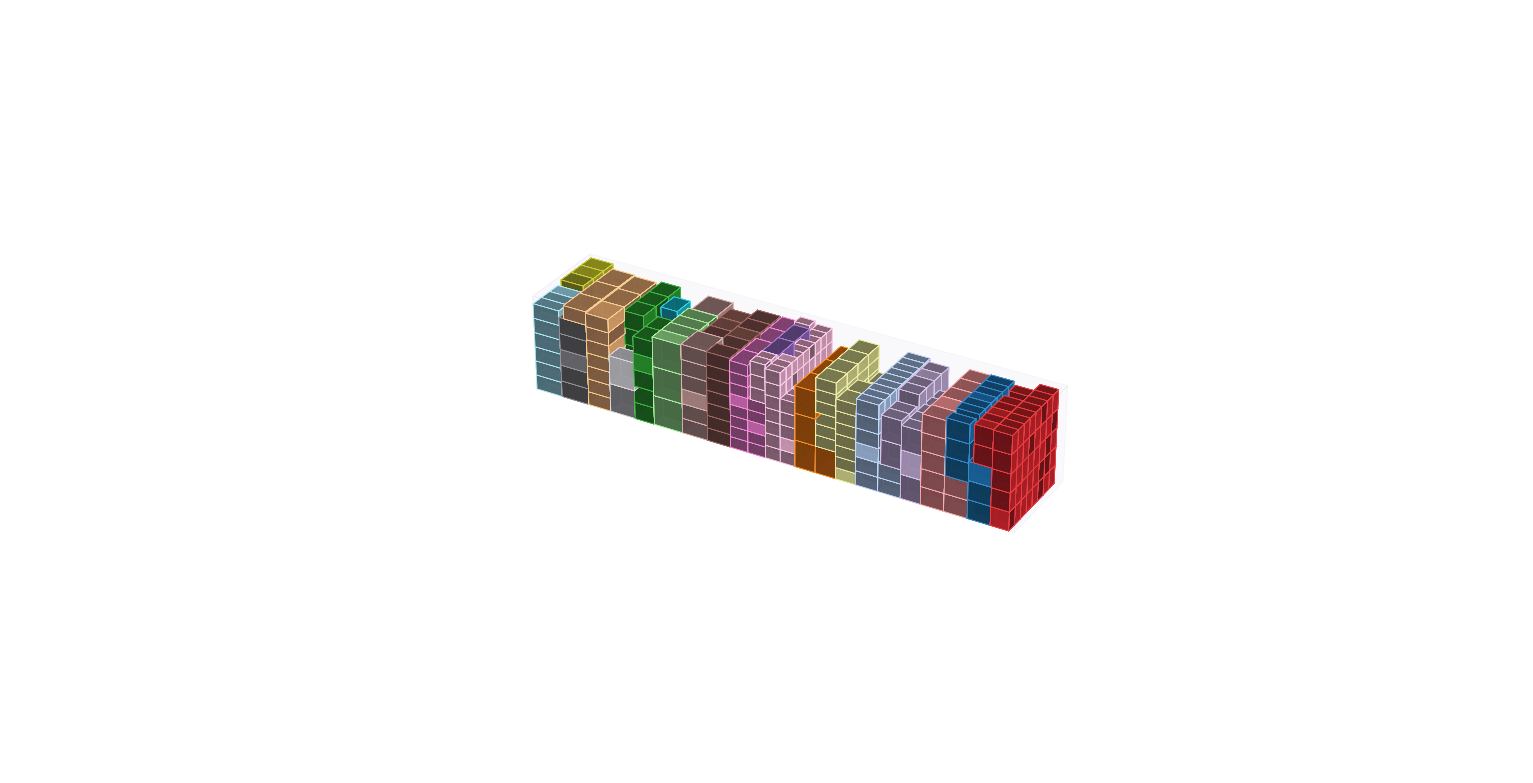
\includegraphics[width=0.8\textwidth]{Figures/ejemplo_solucion.eps}
    \caption{Ejemplo de una solución final generada por el algoritmo genético}
    \label{fig:ejemplo_solucion}
\end{figure}

\subsection{Resultados y análisis}

En esta sección se presentan y analizan los resultados obtenidos del experimento computacional. Los resultados se agrupan en función de las mejoras que incorporan los algoritmos (M0, M1, M2, M3 y M4) y el tipo de instancia (5T, 10T, 20T, 30T, 40T, 50T). Se evalúan dos métricas principales: el beneficio que aporta la solución obtenida y el tiempo de ejecución.

El beneficio obtenido por las soluciones indica qué tan bueno es el resultado final obtenido en comparación con la población inicial. Por otro lado, el tiempo de ejecución mide cuánto tiempo tarda el algoritmo en encontrar la mejor solución. También a partir de estas métricas se calcula el rendimiento de los algoritmos mejorados propuestos, que indica el incremento porcentual en la calidad de las soluciones por cada unidad de tiempo. Con estos resultados, se evalúa y se compara la eficacia de los algoritmos propuestos.

\subsubsection{Calidad de las soluciones: beneficio obtenido}

Dado que queremos comparar no sólo el comportamiento de los diferentes mecanismos de mejora (M1, M2, M3, M4), sino también estudiar cómo varía un mismo mecanismo al incrementar la complejidad de las instancias (5T, 10T, $\cdot$, 50T), se ha optado por elegir como medida de comparación el porcentaje de mejora que obtiene el algoritmo con respecto a la mejor de las soluciones de la población inicial, que al ser común para todos los algoritmos mejorados, permite una comparación justa.

El porcentaje del incremento del beneficio se calcula por conjunto de tipos de cajas respecto al los algoritmos mejorados propuestos. Los resultados promediados sobre las 25 instancias se muestran en la Tabla \ref{tab:valor_aportado}, presentando el promedio y la desviación estándar para cada caso.

\begin{table}[H]
    \centering
    \caption{Comparación de soluciones según el mecanismo de mejora empleado}
    \label{tab:valor_aportado}
    \begin{tabular}{|c|c|c|c|c|c|c|c|c|c|c|}
        \hline
        \multirow{2}{*}{\textbf{Tipo de Caja}} & \multicolumn{2}{c|}{\textbf{M0}} & \multicolumn{2}{c|}{\textbf{M1}} & \multicolumn{2}{c|}{\textbf{M2}} & \multicolumn{2}{c|}{\textbf{M3}} & \multicolumn{2}{c|}{\textbf{M4}}                                                                             \\ \cline{2-11}
                                               & \textbf{media}                   & \textbf{sd}                      & \textbf{media}                   & \textbf{sd}                      & \textbf{media}                   & \textbf{sd} & \textbf{media} & \textbf{sd} & \textbf{media} & \textbf{sd} \\ \hline
        5T                                     & 9.3\%                            & 3.7                              & 10.5\%                           & 4.1                              & 10.4\%                           & 4.1         & 10.0\%         & 4.1         & 9.9\%          & 4.1         \\ \hline
        10T                                    & 18.5\%                           & 6.0                              & 20.9\%                           & 6.1                              & 20.6\%                           & 5.9         & 20.2\%         & 6.1         & 19.0\%         & 5.9         \\ \hline
        20T                                    & 27.2\%                           & 6.5                              & 33.1\%                           & 6.6                              & 32.1\%                           & 6.5         & 31.6\%         & 6.6         & 28.3\%         & 7.0         \\ \hline
        30T                                    & 29.0\%                           & 7.8                              & 37.8\%                           & 8.7                              & 37.2\%                           & 8.9         & 34.9\%         & 7.9         & 31.8\%         & 8.1         \\ \hline
        40T                                    & 28.6\%                           & 8.3                              & 44.5\%                           & 9.8                              & 43.1\%                           & 10.1        & 42.2\%         & 9.8         & 35.1\%         & 9.7         \\ \hline
        50T                                    & 35.2\%                           & 9.4                              & 56.7\%                           & 12.6                             & 54.6\%                           & 12.5        & 52.1\%         & 13.2        & 46.4\%         & 12.3        \\ \hline
    \end{tabular}
\end{table}

Como se observa en la Tabla \ref{tab:valor_aportado}, todos los algoritmos propuestos (M1, M2, M3 y M4) superan a la versión original del algoritmo (M0) en términos de beneficio aportado por las soluciones obtenidas. Los algoritmo M1 y M2, que se aplican a toda la población, muestran los mejores resultados en todos los casos, aumentando la calidad de las soluciones en comparación con las demás versiones de mejora. También se observa que el beneficio aportado por las soluciones aumenta a medida que se incrementa el número de tipos de cajas a llenar, esto debido a que mientras mayor sean los tipos de cajas, el problema se vuelve más complejo y las soluciones iniciales tienden a ser peores lo que permite que los algoritmos mejorados tengan un mayor impacto. Esto se puede observar en la Figura \ref{fig:valores}.

\begin{figure}[H]
    \centering
    \includesvg[width=0.8\textwidth]{Figures/improvement.svg}
    \caption{Comparación de soluciones según el mecanismo de mejora empleado}
    \label{fig:valores}
\end{figure}


La Figura \ref{fig:valores} muestra el incremento del beneficio aportado en porcentaje, por las soluciones obtenidas para cada versión de los algoritmos (M0, ..., M4) y conjunto de tipos de cajas (5T, ..., 50T). Se observa que los algoritmos mejorados M1 y M2 presentan un mayor beneficio aportado en comparación con M0, M3 y M4. Por otro lado, se destaca que cuando la complejidad del problema no es muy alta (5T y 10T), todos los algoritmos presentan desempeños similares, pero a medida que la complejidad aumenta, se observa una clara diferencia entre los distintos mecanismos de mejora de las soluciones.

\subsubsection{Tiempo de ejecución}

El tiempo de ejecución es una métrica crucial para evaluar la eficiencia de los algoritmos genéticos, debido a que no se puede prever cuánto tiempo tomará encontrar la mejor solución. En este experimento, se ha tomado el tiempo de ejecución hasta el momento en el que algoritmo ya no pudo incrementar su beneficio, dentro de los cinco minutos de límite establecidos. Cada medida es tomada para cada versión de los algoritmos (M0, ..., M4) y conjunto de tipos de cajas (5T, ..., 50T), con el objetivo de evaluar el impacto de los mecanismos de mejora en el tiempo de ejecución de los algoritmos.

Se propusieron las mejoras M3 y M4 con la expectativa de reducir el tiempo de ejecución en comparación con M2, sin comprometer demasiado la calidad de las soluciones. Si bien M3 aplica la misma estrategia de mejora al final del llenado similar M2, la diferencia es que aplica dicha mejora solo a la mitad de la población en cada iteración, mientras que M4 la aplica solo al mejor individuo de cada iteración. Es crucial evaluar si estas mejoras efectivamente logran su objetivo de reducir el tiempo de ejecución y si logran mantener la calidad de las soluciones obtenidas.

Cada ejecución se realiza con un conjunto de tipos de cajas (5T, ... 50T) y una versión del algoritmo mejorado específico (M0, ..., M4). Debido a que ha sido establecido un límite de tiempo de cinco minutos para cada ejecución, se registra el tiempo que cada evaluación tarda en encontrar su mejor solución.

En la Tabla \ref{tab:tiempo}, se muestra el tiempo promedio en encontrar la mejor solución (en segundos), junto a la desviación estándar, para cada mecanismo de mejora y conjunto de tipos de cajas.

\begin{table}[H]
    \centering
    \caption{Tiempo promedio en encontrar la mejor solución}
    \label{tab:tiempo}
    \begin{tabular}{|c|c|c|c|c|c|c|c|c|c|c|}
        \hline
        \multirow{2}{*}{\textbf{Tipo de Caja}} & \multicolumn{2}{c|}{\textbf{M0}} & \multicolumn{2}{c|}{\textbf{M1}} & \multicolumn{2}{c|}{\textbf{M2}} & \multicolumn{2}{c|}{\textbf{M3}} & \multicolumn{2}{c|}{\textbf{M4}}                                                                             \\ \cline{2-11}
                                               & \textbf{media}                   & \textbf{sd}                      & \textbf{media}                   & \textbf{sd}                      & \textbf{media}                   & \textbf{sd} & \textbf{media} & \textbf{sd} & \textbf{media} & \textbf{sd} \\ \hline
        5T                                     & 71.4                             & 72.4                             & 23.7                             & 47.6                             & 56.9                             & 71.1        & 33.6           & 63.5        & 39.3           & 47.9        \\ \hline
        10T                                    & 146.0                            & 85.3                             & 72.5                             & 69.2                             & 102.1                            & 87.9        & 61.1           & 59.8        & 117.5          & 85.8        \\ \hline
        20T                                    & 214.4                            & 56.4                             & 89.0                             & 72.6                             & 145.9                            & 62.6        & 188.0          & 79.7        & 166.8          & 70.8        \\ \hline
        30T                                    & 263.1                            & 36.3                             & 183.8                            & 73.9                             & 175.4                            & 81.9        & 186.8          & 70.4        & 231.9          & 48.9        \\ \hline
        40T                                    & 266.2                            & 34.0                             & 208.4                            & 70.0                             & 224.0                            & 50.9        & 244.0          & 49.1        & 238.3          & 54.2        \\ \hline
        50T                                    & 257.0                            & 42.6                             & 244.3                            & 49.2                             & 228.5                            & 61.3        & 251.7          & 36.4        & 250.5          & 51.6        \\ \hline
    \end{tabular}
\end{table}

La Tabla \ref{tab:tiempo} muestra que las mejoras introducidas M1, M2, M3 y M4, a pesar de que requieren tiempo adicional para realizar las operaciones de mejora, reducen ligeramente el tiempo necesario para encontrar la mejor solución en comparación con M0. Esto se debe a que las mejoras permiten que el algoritmo genético encuentre mejores soluciones en cada iteración. Sin embargo, también se observa una tendencia al aumento del tiempo en llegar a la mejor solución a medida que se incrementa el número de tipos de cajas a llenar, lo que se debe a la mayor complejidad del problema. Incluso los valores cercanos a 300 segundos (5 minutos) podría indicar que el algoritmo podría encontrar una solución mejor con más tiempo disponible. Los datos de esta tabla se han representado, para mayor claridad, en la Figura \ref{fig:tiempos}.

\begin{figure}[H]
    \centering
    \includesvg[width=0.8\textwidth]{Figures/tiempos.svg}
    \caption{Tiempo promedio en encontrar la mejor solución}
    \label{fig:tiempos}
\end{figure}

La Figura \ref{fig:tiempos} destaca que el algoritmo mejorado M1 presenta en promedio el menor tiempo en encontrar su mejor solución, en comparación con los otros casos, seguida de M2 y M3 en algunas situaciones. La versión original del algoritmo sin mejoras, M0, muestra un tiempo de de encontrar su mejor solución, significativamente mayor en comparación con las versiones mejoradas. Esto confirma que las mejoras propuestas permiten que el algoritmo genético llegue a sus mejores soluciones de modo más rápido.

También se puede evaluar el tiempo que cada algoritmo necesita para evaluar una generación en una población de 100 individuos. Esto se calcula dividiendo el tiempo total de ejecución, que es de 300 segundos fijos para todos los métodos, por la cantidad de generaciones realizadas. Así obtenemos una idea del tiempo que cada algoritmo requiere para evaluar una generación. En la Figura \ref{fig:tiempo_generacion}, se muestra el tiempo promedio en milisegundos que toma cada algoritmo para evaluar una generación.

\begin{figure}[H]
    \centering
    \includesvg[width=0.8\textwidth]{Figures/tiempo_generacion.svg}
    \caption{Tiempo promedio en evaluar una población}
    \label{fig:tiempo_generacion}
\end{figure}

La Figura \ref{fig:tiempo_generacion} confirma que los algoritmos mejorados M1, M2, M3 y M4 necesitan más tiempo para evaluar una generación en comparación con la versión del algoritmo sin mejoras M0. Esto se debe a que los algoritmos mejorados requieren tiempo adicional para evaluar los espacios libres que se pueden completar con cajas disponibles. Sin embargo, como se ha mostrado en los gráficos anteriores, los algoritmos mejorados también permiten que el algoritmo genético encuentre sus mejores soluciones más rápidamente, lo que compensa el tiempo adicional requerido para realizar las operaciones de mejora en los algoritmos.

\subsubsection{Rendimiento}

Para proporcionar una visión clara del impacto de los algoritmos mejorados, se presenta un análisis comparativo del rendimiento, definido como el \textbf{incremento porcentual en la calidad de las soluciones por cada unidad de tiempo}. La Figura \ref{fig:rendimiento} muestra el rendimiento de los algoritmos propuestos en términos de calidad de las soluciones y tiempo de ejecución.

\begin{figure}[H]
    \centering
    \includesvg[width=0.8\textwidth]{Figures/rendimiento.svg}
    \caption{Rendimiento de los algoritmos propuestos}
    \label{fig:rendimiento}
\end{figure}

Las líneas de la Figura \ref{fig:rendimiento} se pueden interpretar como cuanto beneficio en porcentaje se gana por cada segundo de tiempo de ejecución. Por ejemplo usando 40 tipos de cajas (40T), la versión del algoritmo sin mejoras, ha obtenido en promedio, un incremento aproximado de 0.22\% en cada segundo de ejecución, mientras que la versión mejorada del algoritmo, ha obtenido un incremento de 0.3\% en cada segundo de ejecución. En general, se observa que el algoritmo mejorado M1 proporciona el mayor incremento porcentual en la calidad de las soluciones por cada segundo, seguida de M2 y M3 en algunas situaciones. La versión original del algoritmo sin mejoras, M0, muestra un rendimiento significativamente menor en comparación con las versiones mejoradas.

\subsection{Evaluando el progreso de las soluciones}

Para evaluar el progreso de las soluciones a lo largo de las generaciones, se analiza el beneficio aportado por las soluciones obtenidas durante todo el tiempo de ejecución. Este análisis se centra exclusivamente en la mejora M1, dado que presenta el mejor rendimiento en términos de calidad de las soluciones y tiempo en encontrar su mejor solución. Además, se incluye en el gráfico la versión sin mejoras (M0) para mostrar la diferencia en ambos casos. Además, para simplificar el análisis, se considera solo algunas instancias representativas (10T, 30T, 50T).

En la Figura \ref{fig:progreso}, se muestra el progreso de las soluciones obtenidas por M0 y M1 en las instancias de prueba con 10, 30 y 50 tipos de cajas (10T, 30T, 50T). En esta gráfica, cuando una linea se hace horizontal, puede interpretarse como que el algoritmo converge o ha encontrado su mejor solución, puesto que ya a no ha sido capaz de encontrar mejores soluciones en un elevado número de iteraciones (o tiempo de ejecución).

\begin{figure}[H]
    \centering
    \includesvg[width=0.9\textwidth]{Figures/progreso.svg}
    \caption{Progreso de las soluciones obtenidas por M0 y M1 para 10T, 30T, 50T}
    \label{fig:progreso}
\end{figure}

La Figura \ref{fig:progreso} muestra que M1 logra superar a M0 en términos de calidad de las soluciones en todas las instancias de prueba. También, se observa que M1 encuentra su mejor solución más rápidamente, además, son soluciones de mejor calidad en comparación con M0. Por otro lado, M0 muestra un progreso más lento en comparación con M1.

Por ejemplo las líneas puntuadas, que son las versiones del algoritmo sin mejora M0, se puede apreciar que siguen tendiendo una tendencia de crecimiento lo que indica que aún no encuentran su mejor solución, mientras que la línea sólida roja (Algoritmo M1 con 10 tipos), ha encontrado su mejor solución en un aproximado de 10 segundos, luego se mantuvo en horizontal debido a que ya no ha podido encontrar mejores soluciones. De modo similar la línea sólida azul (Algoritmo M1 con 30 tipos) que ha tardado un aproximado de 100 segundos en encontrar su mejor solución, ya que luego se mantuvo horizontal. Para el caso de la línea morada (Algoritmo M1 con 50 tipos) se puede ver que la línea continúa con una tendencia creciente, lo que indica que todavía sigue encontrando mejores soluciones y  necesita más de cinco minutos para poder encontrar su mejor solución.

Esto confirma que el algoritmo mejorado M1 permite que el algoritmo genético encuentre su mejor solución más rápidamente y obtenga soluciones de mayor calidad en menor tiempo en comparación con la versión sin mejoras. También es importante destacar que a medida que se incrementa el número de tipos de cajas a llenar, la línea de convergencia se pierde, lo que indica que posiblemente en esos casos el algoritmo necesita usar otros parámetros como un mayor tiempo para encontrar la mejor solución.

Por último, es importante resaltar que la mejora M1 es la que muestra mejor rendimiento en términos de calidad de las soluciones y tiempo en encontrar su mejor solución, en la mayoría de evaluaciones con diferentes tipos de cajas, aunque este algoritmo necesite más tiempo que el resto para evaluar una generación completa. M2 y M3 presentan un rendimiento similar en algunas situaciones, con M2 destacando en términos de calidad de las soluciones y M3 en términos de tiempo de ejecución. M4 presenta el peor rendimiento en términos de calidad de las soluciones y tiempo de su línea de convergencia en la mayoría de evaluaciones con diferentes tipos de cajas.









\newpage








\section{Conclusiones}

En este trabajo, se ha abordado el problema del llenado de contenedores con paquetes heterogéneos bajo restricciones prácticas derivadas de un caso de uso real en el contexto de carga manual. A continuación, se resumen las conclusiones más relevantes:

\begin{itemize}
    \item \textbf{Método de solución basado en una metaheurística:} Se propuso un algoritmo genético que considera las restricciones prácticas del llenado manual de contenedores. La codificación de soluciones incluye la secuencia de llenado, el tipo de caja, la rotación y la cantidad de paquetes por cada tipo, lo cual facilita la generación de soluciones factibles y la evaluación de su calidad.

    \item \textbf{Mejoras en el proceso de llenado:} Se han implementado 5 versiones del algoritmo, que difieren en los mecanismos de mejora de las soluciones, durante el proceso de imitación de llenado manual. Todas estas mejoras demostraron ser efectivas para aumentar la calidad de las soluciones y reducir el tiempo en encontrar las mejores soluciones de los algoritmos genéticos.

    \item \textbf{Evaluación con diferentes tipos de cajas:} Se ha llevado a cabo un extenso experimento computacional y para ello se han generado 6 conjuntos de problemas que difieren en el número de tipos de cajas que tienen. para evaluar el rendimiento de los algoritmos genéticos. Los resultados demostraron que las versiones M1 y M2 de los algoritmos genéticos mejorados han sido capaz de manejar eficientemente instancias con diferentes grados de complejidad y diversidad.

    \item \textbf{Rendimiento del algoritmo genético:} Los experimentos computacionales mostraron que los algoritmos con mejoras propuestas (M1 y M2) permiten encontrar las mejores soluciones más rápidamente, además de ser soluciones de mejor calidad en comparación con la versión sin mejoras (M0). En particular, M1 ha resultado ser la más efectiva en términos de rendimiento y tiempo de ejecución, destacando en instancias con mayor número de tipos de cajas (20T, 40T).

    \item \textbf{Impacto en el tiempo de ejecución:} Aunque las mejoras introducidas aumentan ligeramente el tiempo necesario para evaluar cada generación, el tiempo total de ejecución se reduce debido a una convergencia más rápida hacia soluciones de alta calidad. Esto hace que las mejoras sean eficientes tanto en términos de calidad de soluciones como de tiempo de ejecución.
\end{itemize}

En conclusión, el algoritmo genético mejorado presentado en este trabajo proporciona una solución efectiva y eficiente para el problema del llenado de contenedores con paquetes heterogéneos bajo restricciones prácticas. Las mejoras introducidas permiten obtener soluciones de alta calidad en menor tiempo, lo cual es crucial en contextos industriales donde la eficiencia y la reducción de costos son primordiales.

\subsection{Futuras líneas de investigación}

A partir de los resultados obtenidos y las limitaciones observadas, se identifican varias futuras líneas de investigación:

\begin{itemize}
    \item \textbf{Extensión a múltiples contenedores:} Aunque este trabajo se ha centrado en un único contenedor, una extensión natural sería abordar el problema de llenado de múltiples contenedores, lo cual es común en aplicaciones reales de logística y transporte.

    \item \textbf{Consideración de más restricciones prácticas:} Incluir restricciones adicionales, como imponer un mínimo de cantidad para ciertos tipos de paquetes, agregar una dimensión de prioridad entre los tipos, o considerar el balanceo del peso dentro del contenedor, podría aumentar la aplicabilidad del algoritmo propuesto en escenarios más complejos.

    \item \textbf{Optimización de hiperparámetros:} Realizar un estudio más detallado de los hiperparámetros del algoritmo genético, como la probabilidad de mutación y cruce, el tamaño de la población, y el número de generaciones, para determinar su impacto en el rendimiento y la calidad de las soluciones obtenidas.

    \item \textbf{Comparación con otros enfoques metaheurísticos:} Aunque se ha empleado un algoritmo genético, sería interesante comparar su rendimiento con otros enfoques metaheurísticos como algoritmos de enjambre de partículas (PSO), algoritmos de recocido simulado o técnicas híbridas que combinen varias metodologías.

    \item \textbf{Implementación en sistemas reales:} Probar e implementar el algoritmo en sistemas de soporte de decisiones logísticas y de transporte a escala real permitiría validar su efectividad y eficiencia en situaciones prácticas, proporcionando además retroalimentación valiosa para futuras mejoras.

    \item \textbf{Estudio de la implantación del sistema en la empresa:} Estudiar el impacto que esta metodología tendría en la empresa, comparando los resultados con los que está ahora mismo obteniendo la empresa.

    \item \textbf{Optimización en tiempo real:} Desarrollar versiones optimizadas del algoritmo que puedan operar en tiempo real, ajustándose dinámicamente a cambios en las condiciones de carga y disponibilidad de paquetes, podría mejorar aún más su utilidad práctica en entornos de logística en tiempo real.
\end{itemize}

En resumen, el problema del llenado de contenedores con paquetes heterogéneos es un desafío logístico complejo debido a las restricciones prácticas. El algoritmo genético propuesto en este trabajo ofrece una solución efectiva y eficiente para abordar este problema, y las mejoras introducidas permiten obtener soluciones de alta calidad en tiempos reducidos. Las futuras líneas de investigación identificadas apuntan a mejorar y extender el alcance del algoritmo, así como a explorar su aplicabilidad en contextos industriales y de transporte reales.








\newpage

\addcontentsline{toc}{section}{\refname}

\printbibliography

\end{document}